
\subsection{Visualization using rooted trees}


There is another---more graphical---way of describing the Stasheff identities, and this is done by \emph{rooted trees}\index{Rooted tree}. A rooted tree is a graph with a fixed node at the bottom (which we call the root), and where every other two nodes are connected by no more than one line. An example is the following graph.


% Single rooted tree in the form of m_2


\begin{center}
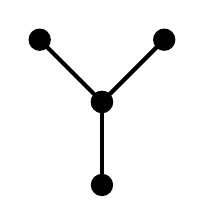
\begin{tikzpicture}[x=0.75pt,y=0.75pt,yscale=-1,xscale=1]
%uncomment if require: \path (0,419); %set diagram left start at 0, and has height of 419

%Straight Lines [id:da8201192265850832] 
\draw [line width=1.5]    (90,60) -- (120,90) ;
\draw [shift={(120,90)}, rotate = 45] [color={rgb, 255:red, 0; green, 0; blue, 0 }  ][fill={rgb, 255:red, 0; green, 0; blue, 0 }  ][line width=1.5]      (0, 0) circle [x radius= 4.36, y radius= 4.36]   ;
\draw [shift={(90,60)}, rotate = 45] [color={rgb, 255:red, 0; green, 0; blue, 0 }  ][fill={rgb, 255:red, 0; green, 0; blue, 0 }  ][line width=1.5]      (0, 0) circle [x radius= 4.36, y radius= 4.36]   ;
%Straight Lines [id:da6726062790054357] 
\draw [line width=1.5]    (120,90) -- (150,60) ;
\draw [shift={(150,60)}, rotate = 315] [color={rgb, 255:red, 0; green, 0; blue, 0 }  ][fill={rgb, 255:red, 0; green, 0; blue, 0 }  ][line width=1.5]      (0, 0) circle [x radius= 4.36, y radius= 4.36]   ;
%Straight Lines [id:da7863057024778404] 
\draw [line width=1.5]    (120,130) -- (120,90) ;
\draw [shift={(120,90)}, rotate = 270] [color={rgb, 255:red, 0; green, 0; blue, 0 }  ][fill={rgb, 255:red, 0; green, 0; blue, 0 }  ][line width=1.5]      (0, 0) circle [x radius= 4.36, y radius= 4.36]   ;
\draw [shift={(120,130)}, rotate = 270] [color={rgb, 255:red, 0; green, 0; blue, 0 }  ][fill={rgb, 255:red, 0; green, 0; blue, 0 }  ][line width=1.5]      (0, 0) circle [x radius= 4.36, y radius= 4.36]   ;
\end{tikzpicture}
\end{center}

The top vertices are called the leaves of the tree. 

We can use these to represent our higher operations. For example---if the above graph is read from top to bottom---it can be thought of as an operation that takes in two elements, and produces just one. This is exactly what $m_2$ does in an $\A$-algebra, hence the reason we can use them. The following graphs represents $m_1, m_2, m_3$ and $m_4$ respectively. 


% 4 Rooted trees in the form of m_1, m_2, m_3, m_4


\begin{center}
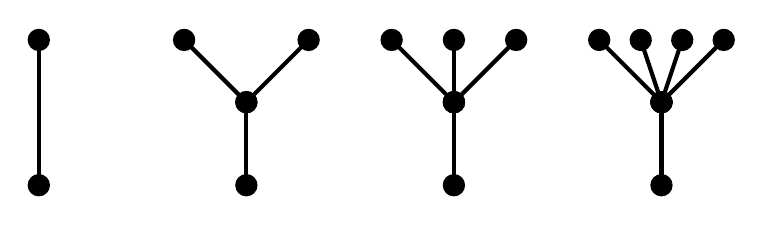
\begin{tikzpicture}[x=0.75pt,y=0.75pt,yscale=-1,xscale=1]
%uncomment if require: \path (0,419); %set diagram left start at 0, and has height of 419

%Straight Lines [id:da7863057024778404] 
\draw [line width=1.5]    (120,130) -- (120,102) -- (120,60) ;
\draw [shift={(120,60)}, rotate = 270] [color={rgb, 255:red, 0; green, 0; blue, 0 }  ][fill={rgb, 255:red, 0; green, 0; blue, 0 }  ][line width=1.5]      (0, 0) circle [x radius= 4.36, y radius= 4.36]   ;
\draw [shift={(120,130)}, rotate = 270] [color={rgb, 255:red, 0; green, 0; blue, 0 }  ][fill={rgb, 255:red, 0; green, 0; blue, 0 }  ][line width=1.5]      (0, 0) circle [x radius= 4.36, y radius= 4.36]   ;
%Straight Lines [id:da3527709376157697] 
\draw [line width=1.5]    (190,60) -- (220,90) ;
\draw [shift={(220,90)}, rotate = 45] [color={rgb, 255:red, 0; green, 0; blue, 0 }  ][fill={rgb, 255:red, 0; green, 0; blue, 0 }  ][line width=1.5]      (0, 0) circle [x radius= 4.36, y radius= 4.36]   ;
\draw [shift={(190,60)}, rotate = 45] [color={rgb, 255:red, 0; green, 0; blue, 0 }  ][fill={rgb, 255:red, 0; green, 0; blue, 0 }  ][line width=1.5]      (0, 0) circle [x radius= 4.36, y radius= 4.36]   ;
%Straight Lines [id:da5026094070566995] 
\draw [line width=1.5]    (220,90) -- (250,60) ;
\draw [shift={(250,60)}, rotate = 315] [color={rgb, 255:red, 0; green, 0; blue, 0 }  ][fill={rgb, 255:red, 0; green, 0; blue, 0 }  ][line width=1.5]      (0, 0) circle [x radius= 4.36, y radius= 4.36]   ;
%Straight Lines [id:da49384351285853745] 
\draw [line width=1.5]    (220,130) -- (220,90) ;
\draw [shift={(220,90)}, rotate = 270] [color={rgb, 255:red, 0; green, 0; blue, 0 }  ][fill={rgb, 255:red, 0; green, 0; blue, 0 }  ][line width=1.5]      (0, 0) circle [x radius= 4.36, y radius= 4.36]   ;
\draw [shift={(220,130)}, rotate = 270] [color={rgb, 255:red, 0; green, 0; blue, 0 }  ][fill={rgb, 255:red, 0; green, 0; blue, 0 }  ][line width=1.5]      (0, 0) circle [x radius= 4.36, y radius= 4.36]   ;
%Straight Lines [id:da4025202167828019] 
\draw [line width=1.5]    (290,60) -- (320,90) ;
\draw [shift={(320,90)}, rotate = 45] [color={rgb, 255:red, 0; green, 0; blue, 0 }  ][fill={rgb, 255:red, 0; green, 0; blue, 0 }  ][line width=1.5]      (0, 0) circle [x radius= 4.36, y radius= 4.36]   ;
\draw [shift={(290,60)}, rotate = 45] [color={rgb, 255:red, 0; green, 0; blue, 0 }  ][fill={rgb, 255:red, 0; green, 0; blue, 0 }  ][line width=1.5]      (0, 0) circle [x radius= 4.36, y radius= 4.36]   ;
%Straight Lines [id:da1762723390926908] 
\draw [line width=1.5]    (320,90) -- (350,60) ;
\draw [shift={(350,60)}, rotate = 315] [color={rgb, 255:red, 0; green, 0; blue, 0 }  ][fill={rgb, 255:red, 0; green, 0; blue, 0 }  ][line width=1.5]      (0, 0) circle [x radius= 4.36, y radius= 4.36]   ;
%Straight Lines [id:da426516312690572] 
\draw [line width=1.5]    (320,130) -- (320,90) ;
\draw [shift={(320,90)}, rotate = 270] [color={rgb, 255:red, 0; green, 0; blue, 0 }  ][fill={rgb, 255:red, 0; green, 0; blue, 0 }  ][line width=1.5]      (0, 0) circle [x radius= 4.36, y radius= 4.36]   ;
\draw [shift={(320,130)}, rotate = 270] [color={rgb, 255:red, 0; green, 0; blue, 0 }  ][fill={rgb, 255:red, 0; green, 0; blue, 0 }  ][line width=1.5]      (0, 0) circle [x radius= 4.36, y radius= 4.36]   ;
%Straight Lines [id:da25638621797362715] 
\draw [line width=1.5]    (390,60) -- (420,90) ;
\draw [shift={(420,90)}, rotate = 45] [color={rgb, 255:red, 0; green, 0; blue, 0 }  ][fill={rgb, 255:red, 0; green, 0; blue, 0 }  ][line width=1.5]      (0, 0) circle [x radius= 4.36, y radius= 4.36]   ;
\draw [shift={(390,60)}, rotate = 45] [color={rgb, 255:red, 0; green, 0; blue, 0 }  ][fill={rgb, 255:red, 0; green, 0; blue, 0 }  ][line width=1.5]      (0, 0) circle [x radius= 4.36, y radius= 4.36]   ;
%Straight Lines [id:da44171571517014097] 
\draw [line width=1.5]    (420,90) -- (450,60) ;
\draw [shift={(450,60)}, rotate = 315] [color={rgb, 255:red, 0; green, 0; blue, 0 }  ][fill={rgb, 255:red, 0; green, 0; blue, 0 }  ][line width=1.5]      (0, 0) circle [x radius= 4.36, y radius= 4.36]   ;
%Straight Lines [id:da05493894156577439] 
\draw [line width=1.5]    (420,130) -- (420,90) ;
\draw [shift={(420,90)}, rotate = 270] [color={rgb, 255:red, 0; green, 0; blue, 0 }  ][fill={rgb, 255:red, 0; green, 0; blue, 0 }  ][line width=1.5]      (0, 0) circle [x radius= 4.36, y radius= 4.36]   ;
\draw [shift={(420,130)}, rotate = 270] [color={rgb, 255:red, 0; green, 0; blue, 0 }  ][fill={rgb, 255:red, 0; green, 0; blue, 0 }  ][line width=1.5]      (0, 0) circle [x radius= 4.36, y radius= 4.36]   ;
%Straight Lines [id:da6858869913750809] 
\draw [line width=1.5]    (320,60) -- (320,90) ;
\draw [shift={(320,90)}, rotate = 90] [color={rgb, 255:red, 0; green, 0; blue, 0 }  ][fill={rgb, 255:red, 0; green, 0; blue, 0 }  ][line width=1.5]      (0, 0) circle [x radius= 4.36, y radius= 4.36]   ;
\draw [shift={(320,60)}, rotate = 90] [color={rgb, 255:red, 0; green, 0; blue, 0 }  ][fill={rgb, 255:red, 0; green, 0; blue, 0 }  ][line width=1.5]      (0, 0) circle [x radius= 4.36, y radius= 4.36]   ;
%Straight Lines [id:da8443523560205857] 
\draw [line width=1.5]    (430,60) -- (420,90) ;
\draw [shift={(420,90)}, rotate = 108.43] [color={rgb, 255:red, 0; green, 0; blue, 0 }  ][fill={rgb, 255:red, 0; green, 0; blue, 0 }  ][line width=1.5]      (0, 0) circle [x radius= 4.36, y radius= 4.36]   ;
\draw [shift={(430,60)}, rotate = 108.43] [color={rgb, 255:red, 0; green, 0; blue, 0 }  ][fill={rgb, 255:red, 0; green, 0; blue, 0 }  ][line width=1.5]      (0, 0) circle [x radius= 4.36, y radius= 4.36]   ;
%Straight Lines [id:da17678730528828934] 
\draw [line width=1.5]    (410,60) -- (420,90) ;
\draw [shift={(420,90)}, rotate = 71.57] [color={rgb, 255:red, 0; green, 0; blue, 0 }  ][fill={rgb, 255:red, 0; green, 0; blue, 0 }  ][line width=1.5]      (0, 0) circle [x radius= 4.36, y radius= 4.36]   ;
\draw [shift={(410,60)}, rotate = 71.57] [color={rgb, 255:red, 0; green, 0; blue, 0 }  ][fill={rgb, 255:red, 0; green, 0; blue, 0 }  ][line width=1.5]      (0, 0) circle [x radius= 4.36, y radius= 4.36]   ;
\end{tikzpicture}    
\end{center}

Adding more leaves to the central vertex gives all the other $m_i$'s as well. We can let these trees interact in certain ways in order to produce the Stasheff identities. Let's start with $n=1$. This relation is given by $m_1 m_1=0$, which we can describe with the following rooted tree:


% The rooted tree relation describing the first Stasheff identity

\begin{center}
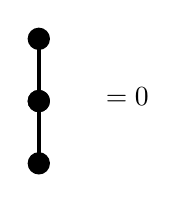
\begin{tikzpicture}[x=0.75pt,y=0.75pt,yscale=-1,xscale=1]
%uncomment if require: \path (0,300); %set diagram left start at 0, and has height of 300

%Straight Lines [id:da5019380442854864] 
\draw [line width=1.5]    (150,180) -- (150,150) ;
\draw [shift={(150,150)}, rotate = 270] [color={rgb, 255:red, 0; green, 0; blue, 0 }  ][fill={rgb, 255:red, 0; green, 0; blue, 0 }  ][line width=1.5]      (0, 0) circle [x radius= 4.36, y radius= 4.36]   ;
\draw [shift={(150,180)}, rotate = 270] [color={rgb, 255:red, 0; green, 0; blue, 0 }  ][fill={rgb, 255:red, 0; green, 0; blue, 0 }  ][line width=1.5]      (0, 0) circle [x radius= 4.36, y radius= 4.36]   ;
%Straight Lines [id:da19340736805161174] 
\draw [line width=1.5]    (150,150) -- (150,120) ;
\draw [shift={(150,120)}, rotate = 270] [color={rgb, 255:red, 0; green, 0; blue, 0 }  ][fill={rgb, 255:red, 0; green, 0; blue, 0 }  ][line width=1.5]      (0, 0) circle [x radius= 4.36, y radius= 4.36]   ;
\draw [shift={(150,150)}, rotate = 270] [color={rgb, 255:red, 0; green, 0; blue, 0 }  ][fill={rgb, 255:red, 0; green, 0; blue, 0 }  ][line width=1.5]      (0, 0) circle [x radius= 4.36, y radius= 4.36]   ;

\draw (181,142.4) node [anchor=north west][inner sep=0.75pt]    {$=0$};

\end{tikzpicture}
\end{center}

Here we have stacked them on top of each other in order to signify that they happen ``after'' each other. We still read from top to bottom, which means that we first do $m_1$, and then $m_1$ again. Note that this rooted tree is the unique way of combining two operations, $m_i, m_j$, such that the combination is an operation that takes in one element and produces one element. 

For $n=2$ we have more than one way of composing the trees, hence the relation must be described by a sum of rooted trees instead. The second relation looks at ways to combine two operations, $m_i, m_j$, in order to form an operation that takes in two elements and produces just one element. There are three ways of doing this, represented by the following three rooted trees:

% Describing the different ways of combining two trees to get two inputs


\begin{center}
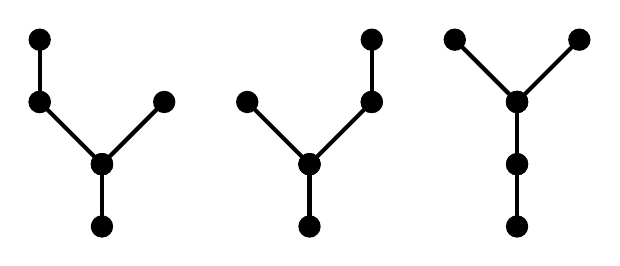
\begin{tikzpicture}[x=0.75pt,y=0.75pt,yscale=-1,xscale=1]
%uncomment if require: \path (0,300); %set diagram left start at 0, and has height of 300

%Straight Lines [id:da8814852158143938] 
\draw [line width=1.5]    (170,180) -- (140,150) ;
\draw [shift={(140,150)}, rotate = 225] [color={rgb, 255:red, 0; green, 0; blue, 0 }  ][fill={rgb, 255:red, 0; green, 0; blue, 0 }  ][line width=1.5]      (0, 0) circle [x radius= 4.36, y radius= 4.36]   ;
\draw [shift={(170,180)}, rotate = 225] [color={rgb, 255:red, 0; green, 0; blue, 0 }  ][fill={rgb, 255:red, 0; green, 0; blue, 0 }  ][line width=1.5]      (0, 0) circle [x radius= 4.36, y radius= 4.36]   ;
%Straight Lines [id:da11602747759122667] 
\draw [line width=1.5]    (140,150) -- (140,120) ;
\draw [shift={(140,120)}, rotate = 270] [color={rgb, 255:red, 0; green, 0; blue, 0 }  ][fill={rgb, 255:red, 0; green, 0; blue, 0 }  ][line width=1.5]      (0, 0) circle [x radius= 4.36, y radius= 4.36]   ;
\draw [shift={(140,150)}, rotate = 270] [color={rgb, 255:red, 0; green, 0; blue, 0 }  ][fill={rgb, 255:red, 0; green, 0; blue, 0 }  ][line width=1.5]      (0, 0) circle [x radius= 4.36, y radius= 4.36]   ;
%Straight Lines [id:da680545812820597] 
\draw [line width=1.5]    (170,180) -- (200,150) ;
\draw [shift={(200,150)}, rotate = 315] [color={rgb, 255:red, 0; green, 0; blue, 0 }  ][fill={rgb, 255:red, 0; green, 0; blue, 0 }  ][line width=1.5]      (0, 0) circle [x radius= 4.36, y radius= 4.36]   ;
\draw [shift={(170,180)}, rotate = 315] [color={rgb, 255:red, 0; green, 0; blue, 0 }  ][fill={rgb, 255:red, 0; green, 0; blue, 0 }  ][line width=1.5]      (0, 0) circle [x radius= 4.36, y radius= 4.36]   ;
%Straight Lines [id:da614958153258419] 
\draw [line width=1.5]    (170,210) -- (170,180) ;
\draw [shift={(170,180)}, rotate = 270] [color={rgb, 255:red, 0; green, 0; blue, 0 }  ][fill={rgb, 255:red, 0; green, 0; blue, 0 }  ][line width=1.5]      (0, 0) circle [x radius= 4.36, y radius= 4.36]   ;
\draw [shift={(170,210)}, rotate = 270] [color={rgb, 255:red, 0; green, 0; blue, 0 }  ][fill={rgb, 255:red, 0; green, 0; blue, 0 }  ][line width=1.5]      (0, 0) circle [x radius= 4.36, y radius= 4.36]   ;
%Straight Lines [id:da2890370558484694] 
\draw [line width=1.5]    (270,180) -- (240,150) ;
\draw [shift={(240,150)}, rotate = 225] [color={rgb, 255:red, 0; green, 0; blue, 0 }  ][fill={rgb, 255:red, 0; green, 0; blue, 0 }  ][line width=1.5]      (0, 0) circle [x radius= 4.36, y radius= 4.36]   ;
\draw [shift={(270,180)}, rotate = 225] [color={rgb, 255:red, 0; green, 0; blue, 0 }  ][fill={rgb, 255:red, 0; green, 0; blue, 0 }  ][line width=1.5]      (0, 0) circle [x radius= 4.36, y radius= 4.36]   ;
%Straight Lines [id:da36602089442829633] 
\draw [line width=1.5]    (300,150) -- (300,120) ;
\draw [shift={(300,120)}, rotate = 270] [color={rgb, 255:red, 0; green, 0; blue, 0 }  ][fill={rgb, 255:red, 0; green, 0; blue, 0 }  ][line width=1.5]      (0, 0) circle [x radius= 4.36, y radius= 4.36]   ;
\draw [shift={(300,150)}, rotate = 270] [color={rgb, 255:red, 0; green, 0; blue, 0 }  ][fill={rgb, 255:red, 0; green, 0; blue, 0 }  ][line width=1.5]      (0, 0) circle [x radius= 4.36, y radius= 4.36]   ;
%Straight Lines [id:da7885321218362338] 
\draw [line width=1.5]    (270,180) -- (300,150) ;
\draw [shift={(300,150)}, rotate = 315] [color={rgb, 255:red, 0; green, 0; blue, 0 }  ][fill={rgb, 255:red, 0; green, 0; blue, 0 }  ][line width=1.5]      (0, 0) circle [x radius= 4.36, y radius= 4.36]   ;
\draw [shift={(270,180)}, rotate = 315] [color={rgb, 255:red, 0; green, 0; blue, 0 }  ][fill={rgb, 255:red, 0; green, 0; blue, 0 }  ][line width=1.5]      (0, 0) circle [x radius= 4.36, y radius= 4.36]   ;
%Straight Lines [id:da9545027465587088] 
\draw [line width=1.5]    (270,210) -- (270,180) ;
\draw [shift={(270,180)}, rotate = 270] [color={rgb, 255:red, 0; green, 0; blue, 0 }  ][fill={rgb, 255:red, 0; green, 0; blue, 0 }  ][line width=1.5]      (0, 0) circle [x radius= 4.36, y radius= 4.36]   ;
\draw [shift={(270,210)}, rotate = 270] [color={rgb, 255:red, 0; green, 0; blue, 0 }  ][fill={rgb, 255:red, 0; green, 0; blue, 0 }  ][line width=1.5]      (0, 0) circle [x radius= 4.36, y radius= 4.36]   ;
%Straight Lines [id:da07994174288427436] 
\draw [line width=1.5]    (370,150) -- (340,120) ;
\draw [shift={(340,120)}, rotate = 225] [color={rgb, 255:red, 0; green, 0; blue, 0 }  ][fill={rgb, 255:red, 0; green, 0; blue, 0 }  ][line width=1.5]      (0, 0) circle [x radius= 4.36, y radius= 4.36]   ;
\draw [shift={(370,150)}, rotate = 225] [color={rgb, 255:red, 0; green, 0; blue, 0 }  ][fill={rgb, 255:red, 0; green, 0; blue, 0 }  ][line width=1.5]      (0, 0) circle [x radius= 4.36, y radius= 4.36]   ;
%Straight Lines [id:da5019380442854864] 
\draw [line width=1.5]    (370,210) -- (370,180) ;
\draw [shift={(370,180)}, rotate = 270] [color={rgb, 255:red, 0; green, 0; blue, 0 }  ][fill={rgb, 255:red, 0; green, 0; blue, 0 }  ][line width=1.5]      (0, 0) circle [x radius= 4.36, y radius= 4.36]   ;
\draw [shift={(370,210)}, rotate = 270] [color={rgb, 255:red, 0; green, 0; blue, 0 }  ][fill={rgb, 255:red, 0; green, 0; blue, 0 }  ][line width=1.5]      (0, 0) circle [x radius= 4.36, y radius= 4.36]   ;
%Straight Lines [id:da16295370354613858] 
\draw [line width=1.5]    (370,150) -- (400,120) ;
\draw [shift={(400,120)}, rotate = 315] [color={rgb, 255:red, 0; green, 0; blue, 0 }  ][fill={rgb, 255:red, 0; green, 0; blue, 0 }  ][line width=1.5]      (0, 0) circle [x radius= 4.36, y radius= 4.36]   ;
\draw [shift={(370,150)}, rotate = 315] [color={rgb, 255:red, 0; green, 0; blue, 0 }  ][fill={rgb, 255:red, 0; green, 0; blue, 0 }  ][line width=1.5]      (0, 0) circle [x radius= 4.36, y radius= 4.36]   ;
%Straight Lines [id:da19340736805161174] 
\draw [line width=1.5]    (370,180) -- (370,150) ;
\draw [shift={(370,150)}, rotate = 270] [color={rgb, 255:red, 0; green, 0; blue, 0 }  ][fill={rgb, 255:red, 0; green, 0; blue, 0 }  ][line width=1.5]      (0, 0) circle [x radius= 4.36, y radius= 4.36]   ;
\draw [shift={(370,180)}, rotate = 270] [color={rgb, 255:red, 0; green, 0; blue, 0 }  ][fill={rgb, 255:red, 0; green, 0; blue, 0 }  ][line width=1.5]      (0, 0) circle [x radius= 4.36, y radius= 4.36]   ;
\end{tikzpicture}    
\end{center}

Note here that we have omitted the identity maps which should be present. If we add these we get for example the following:

% Describing the omittance of identity maps in the drawings

\begin{center}
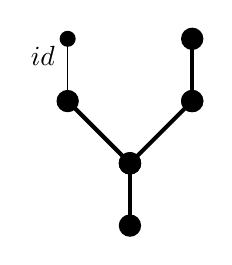
\begin{tikzpicture}[x=0.75pt,y=0.75pt,yscale=-1,xscale=1]
%uncomment if require: \path (0,300); %set diagram left start at 0, and has height of 300

%Straight Lines [id:da3941708866613911] 
\draw [line width=1.5]    (220,140) -- (190,110) ;
\draw [shift={(190,110)}, rotate = 225] [color={rgb, 255:red, 0; green, 0; blue, 0 }  ][fill={rgb, 255:red, 0; green, 0; blue, 0 }  ][line width=1.5]      (0, 0) circle [x radius= 4.36, y radius= 4.36]   ;
\draw [shift={(220,140)}, rotate = 225] [color={rgb, 255:red, 0; green, 0; blue, 0 }  ][fill={rgb, 255:red, 0; green, 0; blue, 0 }  ][line width=1.5]      (0, 0) circle [x radius= 4.36, y radius= 4.36]   ;
%Straight Lines [id:da300120384085371] 
\draw [line width=1.5]    (220,140) -- (250,110) ;
\draw [shift={(250,110)}, rotate = 315] [color={rgb, 255:red, 0; green, 0; blue, 0 }  ][fill={rgb, 255:red, 0; green, 0; blue, 0 }  ][line width=1.5]      (0, 0) circle [x radius= 4.36, y radius= 4.36]   ;
\draw [shift={(220,140)}, rotate = 315] [color={rgb, 255:red, 0; green, 0; blue, 0 }  ][fill={rgb, 255:red, 0; green, 0; blue, 0 }  ][line width=1.5]      (0, 0) circle [x radius= 4.36, y radius= 4.36]   ;
%Straight Lines [id:da14962304311021435] 
\draw [line width=1.5]    (220,170) -- (220,140) ;
\draw [shift={(220,140)}, rotate = 270] [color={rgb, 255:red, 0; green, 0; blue, 0 }  ][fill={rgb, 255:red, 0; green, 0; blue, 0 }  ][line width=1.5]      (0, 0) circle [x radius= 4.36, y radius= 4.36]   ;
\draw [shift={(220,170)}, rotate = 270] [color={rgb, 255:red, 0; green, 0; blue, 0 }  ][fill={rgb, 255:red, 0; green, 0; blue, 0 }  ][line width=1.5]      (0, 0) circle [x radius= 4.36, y radius= 4.36]   ;
%Straight Lines [id:da41279118247571556] 
\draw [line width=1.5]    (250,110) -- (250,80) ;
\draw [shift={(250,80)}, rotate = 270] [color={rgb, 255:red, 0; green, 0; blue, 0 }  ][fill={rgb, 255:red, 0; green, 0; blue, 0 }  ][line width=1.5]      (0, 0) circle [x radius= 4.36, y radius= 4.36]   ;
\draw [shift={(250,110)}, rotate = 270] [color={rgb, 255:red, 0; green, 0; blue, 0 }  ][fill={rgb, 255:red, 0; green, 0; blue, 0 }  ][line width=1.5]      (0, 0) circle [x radius= 4.36, y radius= 4.36]   ;
%Straight Lines [id:da9592865880987089] 
\draw    (190,80) -- (190,110) ;
\draw [shift={(190,80)}, rotate = 90] [color={rgb, 255:red, 0; green, 0; blue, 0 }  ][fill={rgb, 255:red, 0; green, 0; blue, 0 }  ][line width=0.75]      (0, 0) circle [x radius= 3.35, y radius= 3.35]   ;

% Text Node
\draw (171,82.4) node [anchor=north west][inner sep=0.75pt]    {$id$};


\end{tikzpicture}    
\end{center}

For simplicity we omit these identities, as they add a bit of confusion because of their similarity to the $m_1$ operation. So whenever one sees a leaf at a lower level than another, add identities on top until they reach the same height.

In order to produce the second Stasheff identity we need to add these together in the correct way. This correct way, as calculated earlier, is the following:

% Second Stasheff identity using trees, with signs



\begin{center}
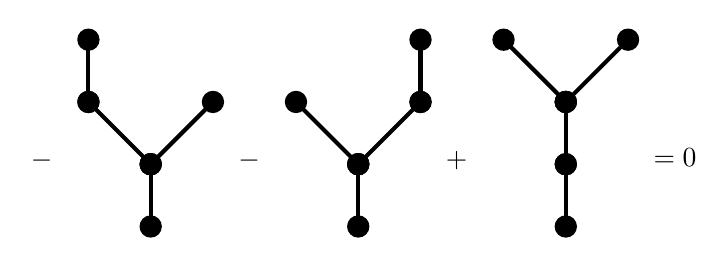
\begin{tikzpicture}[x=0.75pt,y=0.75pt,yscale=-1,xscale=1]
%uncomment if require: \path (0,300); %set diagram left start at 0, and has height of 300

%Straight Lines [id:da31477124000159296] 
\draw [line width=1.5]    (120,140) -- (90,110) ;
\draw [shift={(90,110)}, rotate = 225] [color={rgb, 255:red, 0; green, 0; blue, 0 }  ][fill={rgb, 255:red, 0; green, 0; blue, 0 }  ][line width=1.5]      (0, 0) circle [x radius= 4.36, y radius= 4.36]   ;
\draw [shift={(120,140)}, rotate = 225] [color={rgb, 255:red, 0; green, 0; blue, 0 }  ][fill={rgb, 255:red, 0; green, 0; blue, 0 }  ][line width=1.5]      (0, 0) circle [x radius= 4.36, y radius= 4.36]   ;
%Straight Lines [id:da49139183729214175] 
\draw [line width=1.5]    (120,140) -- (150,110) ;
\draw [shift={(150,110)}, rotate = 315] [color={rgb, 255:red, 0; green, 0; blue, 0 }  ][fill={rgb, 255:red, 0; green, 0; blue, 0 }  ][line width=1.5]      (0, 0) circle [x radius= 4.36, y radius= 4.36]   ;
\draw [shift={(120,140)}, rotate = 315] [color={rgb, 255:red, 0; green, 0; blue, 0 }  ][fill={rgb, 255:red, 0; green, 0; blue, 0 }  ][line width=1.5]      (0, 0) circle [x radius= 4.36, y radius= 4.36]   ;
%Straight Lines [id:da49681202435755245] 
\draw [line width=1.5]    (120,170) -- (120,140) ;
\draw [shift={(120,140)}, rotate = 270] [color={rgb, 255:red, 0; green, 0; blue, 0 }  ][fill={rgb, 255:red, 0; green, 0; blue, 0 }  ][line width=1.5]      (0, 0) circle [x radius= 4.36, y radius= 4.36]   ;
\draw [shift={(120,170)}, rotate = 270] [color={rgb, 255:red, 0; green, 0; blue, 0 }  ][fill={rgb, 255:red, 0; green, 0; blue, 0 }  ][line width=1.5]      (0, 0) circle [x radius= 4.36, y radius= 4.36]   ;
%Straight Lines [id:da3941708866613911] 
\draw [line width=1.5]    (220,140) -- (190,110) ;
\draw [shift={(190,110)}, rotate = 225] [color={rgb, 255:red, 0; green, 0; blue, 0 }  ][fill={rgb, 255:red, 0; green, 0; blue, 0 }  ][line width=1.5]      (0, 0) circle [x radius= 4.36, y radius= 4.36]   ;
\draw [shift={(220,140)}, rotate = 225] [color={rgb, 255:red, 0; green, 0; blue, 0 }  ][fill={rgb, 255:red, 0; green, 0; blue, 0 }  ][line width=1.5]      (0, 0) circle [x radius= 4.36, y radius= 4.36]   ;
%Straight Lines [id:da300120384085371] 
\draw [line width=1.5]    (220,140) -- (250,110) ;
\draw [shift={(250,110)}, rotate = 315] [color={rgb, 255:red, 0; green, 0; blue, 0 }  ][fill={rgb, 255:red, 0; green, 0; blue, 0 }  ][line width=1.5]      (0, 0) circle [x radius= 4.36, y radius= 4.36]   ;
\draw [shift={(220,140)}, rotate = 315] [color={rgb, 255:red, 0; green, 0; blue, 0 }  ][fill={rgb, 255:red, 0; green, 0; blue, 0 }  ][line width=1.5]      (0, 0) circle [x radius= 4.36, y radius= 4.36]   ;
%Straight Lines [id:da14962304311021435] 
\draw [line width=1.5]    (220,170) -- (220,140) ;
\draw [shift={(220,140)}, rotate = 270] [color={rgb, 255:red, 0; green, 0; blue, 0 }  ][fill={rgb, 255:red, 0; green, 0; blue, 0 }  ][line width=1.5]      (0, 0) circle [x radius= 4.36, y radius= 4.36]   ;
\draw [shift={(220,170)}, rotate = 270] [color={rgb, 255:red, 0; green, 0; blue, 0 }  ][fill={rgb, 255:red, 0; green, 0; blue, 0 }  ][line width=1.5]      (0, 0) circle [x radius= 4.36, y radius= 4.36]   ;
%Straight Lines [id:da6955709488854369] 
\draw [line width=1.5]    (320,110) -- (290,80) ;
\draw [shift={(290,80)}, rotate = 225] [color={rgb, 255:red, 0; green, 0; blue, 0 }  ][fill={rgb, 255:red, 0; green, 0; blue, 0 }  ][line width=1.5]      (0, 0) circle [x radius= 4.36, y radius= 4.36]   ;
\draw [shift={(320,110)}, rotate = 225] [color={rgb, 255:red, 0; green, 0; blue, 0 }  ][fill={rgb, 255:red, 0; green, 0; blue, 0 }  ][line width=1.5]      (0, 0) circle [x radius= 4.36, y radius= 4.36]   ;
%Straight Lines [id:da11504103913241726] 
\draw [line width=1.5]    (320,110) -- (350,80) ;
\draw [shift={(350,80)}, rotate = 315] [color={rgb, 255:red, 0; green, 0; blue, 0 }  ][fill={rgb, 255:red, 0; green, 0; blue, 0 }  ][line width=1.5]      (0, 0) circle [x radius= 4.36, y radius= 4.36]   ;
\draw [shift={(320,110)}, rotate = 315] [color={rgb, 255:red, 0; green, 0; blue, 0 }  ][fill={rgb, 255:red, 0; green, 0; blue, 0 }  ][line width=1.5]      (0, 0) circle [x radius= 4.36, y radius= 4.36]   ;
%Straight Lines [id:da004089317473789711] 
\draw [line width=1.5]    (320,140) -- (320,110) ;
\draw [shift={(320,110)}, rotate = 270] [color={rgb, 255:red, 0; green, 0; blue, 0 }  ][fill={rgb, 255:red, 0; green, 0; blue, 0 }  ][line width=1.5]      (0, 0) circle [x radius= 4.36, y radius= 4.36]   ;
\draw [shift={(320,140)}, rotate = 270] [color={rgb, 255:red, 0; green, 0; blue, 0 }  ][fill={rgb, 255:red, 0; green, 0; blue, 0 }  ][line width=1.5]      (0, 0) circle [x radius= 4.36, y radius= 4.36]   ;
%Straight Lines [id:da8569365387106636] 
\draw [line width=1.5]    (90,110) -- (90,80) ;
\draw [shift={(90,80)}, rotate = 270] [color={rgb, 255:red, 0; green, 0; blue, 0 }  ][fill={rgb, 255:red, 0; green, 0; blue, 0 }  ][line width=1.5]      (0, 0) circle [x radius= 4.36, y radius= 4.36]   ;
\draw [shift={(90,110)}, rotate = 270] [color={rgb, 255:red, 0; green, 0; blue, 0 }  ][fill={rgb, 255:red, 0; green, 0; blue, 0 }  ][line width=1.5]      (0, 0) circle [x radius= 4.36, y radius= 4.36]   ;
%Straight Lines [id:da41279118247571556] 
\draw [line width=1.5]    (250,110) -- (250,80) ;
\draw [shift={(250,80)}, rotate = 270] [color={rgb, 255:red, 0; green, 0; blue, 0 }  ][fill={rgb, 255:red, 0; green, 0; blue, 0 }  ][line width=1.5]      (0, 0) circle [x radius= 4.36, y radius= 4.36]   ;
\draw [shift={(250,110)}, rotate = 270] [color={rgb, 255:red, 0; green, 0; blue, 0 }  ][fill={rgb, 255:red, 0; green, 0; blue, 0 }  ][line width=1.5]      (0, 0) circle [x radius= 4.36, y radius= 4.36]   ;
%Straight Lines [id:da5701552758066648] 
\draw [line width=1.5]    (320,170) -- (320,140) ;
\draw [shift={(320,140)}, rotate = 270] [color={rgb, 255:red, 0; green, 0; blue, 0 }  ][fill={rgb, 255:red, 0; green, 0; blue, 0 }  ][line width=1.5]      (0, 0) circle [x radius= 4.36, y radius= 4.36]   ;
\draw [shift={(320,170)}, rotate = 270] [color={rgb, 255:red, 0; green, 0; blue, 0 }  ][fill={rgb, 255:red, 0; green, 0; blue, 0 }  ][line width=1.5]      (0, 0) circle [x radius= 4.36, y radius= 4.36]   ;

% Text Node
\draw (361,131.4) node [anchor=north west][inner sep=0.75pt]    {$=0$};
% Text Node
\draw (61,132.4) node [anchor=north west][inner sep=0.75pt]    {$-$};
% Text Node
\draw (161,132.4) node [anchor=north west][inner sep=0.75pt]    {$-$};
% Text Node
\draw (261,132.4) node [anchor=north west][inner sep=0.75pt]    {$+$};


\end{tikzpicture}    
\end{center}

We can figure out the correct signs by looking at the $r, s, t$ decomposition of $n$. For this particular example---when $n=2$---we have three decompositions
\begin{itemize}
    \item $r=0, s=1, t=1$
    \item $r=1, s=1, t=0$
    \item $r=0, s=2, t=0$
\end{itemize}
These are the ingredients in the sign $(-1)^{r+st}$ which we had in the Stasheff identities. The integer $s$ denotes the operation $m_s$, which we see at the top of the rooted tree. The integer $r$ denotes the position of this top operation, i.e. how far to the right it will be placed on the leaves of the operation at the bottom. The bottom operation will be given by $r+1+t$, i.e. $m_{r+1+t}$. This means that we can read of the correct sign from the composed rooted tree of the two operations. Let's see an example. If we take the middle rooted tree of the ones above, we can read off $r, s, t$ as follows: 

% Describing how to read off the correct sign from the tree



\begin{center}
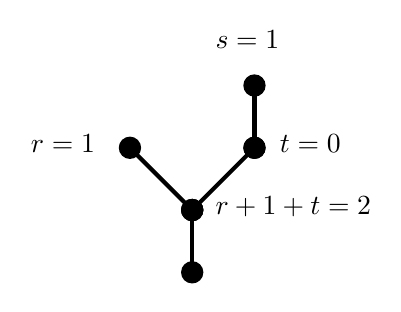
\begin{tikzpicture}[x=0.75pt,y=0.75pt,yscale=-1,xscale=1]
%uncomment if require: \path (0,300); %set diagram left start at 0, and has height of 300

%Straight Lines [id:da3941708866613911] 
\draw [line width=1.5]    (220,140) -- (190,110) ;
\draw [shift={(190,110)}, rotate = 225] [color={rgb, 255:red, 0; green, 0; blue, 0 }  ][fill={rgb, 255:red, 0; green, 0; blue, 0 }  ][line width=1.5]      (0, 0) circle [x radius= 4.36, y radius= 4.36]   ;
\draw [shift={(220,140)}, rotate = 225] [color={rgb, 255:red, 0; green, 0; blue, 0 }  ][fill={rgb, 255:red, 0; green, 0; blue, 0 }  ][line width=1.5]      (0, 0) circle [x radius= 4.36, y radius= 4.36]   ;
%Straight Lines [id:da300120384085371] 
\draw [line width=1.5]    (220,140) -- (250,110) ;
\draw [shift={(250,110)}, rotate = 315] [color={rgb, 255:red, 0; green, 0; blue, 0 }  ][fill={rgb, 255:red, 0; green, 0; blue, 0 }  ][line width=1.5]      (0, 0) circle [x radius= 4.36, y radius= 4.36]   ;
\draw [shift={(220,140)}, rotate = 315] [color={rgb, 255:red, 0; green, 0; blue, 0 }  ][fill={rgb, 255:red, 0; green, 0; blue, 0 }  ][line width=1.5]      (0, 0) circle [x radius= 4.36, y radius= 4.36]   ;
%Straight Lines [id:da14962304311021435] 
\draw [line width=1.5]    (220,170) -- (220,140) ;
\draw [shift={(220,140)}, rotate = 270] [color={rgb, 255:red, 0; green, 0; blue, 0 }  ][fill={rgb, 255:red, 0; green, 0; blue, 0 }  ][line width=1.5]      (0, 0) circle [x radius= 4.36, y radius= 4.36]   ;
\draw [shift={(220,170)}, rotate = 270] [color={rgb, 255:red, 0; green, 0; blue, 0 }  ][fill={rgb, 255:red, 0; green, 0; blue, 0 }  ][line width=1.5]      (0, 0) circle [x radius= 4.36, y radius= 4.36]   ;
%Straight Lines [id:da41279118247571556] 
\draw [line width=1.5]    (250,110) -- (250,80) ;
\draw [shift={(250,80)}, rotate = 270] [color={rgb, 255:red, 0; green, 0; blue, 0 }  ][fill={rgb, 255:red, 0; green, 0; blue, 0 }  ][line width=1.5]      (0, 0) circle [x radius= 4.36, y radius= 4.36]   ;
\draw [shift={(250,110)}, rotate = 270] [color={rgb, 255:red, 0; green, 0; blue, 0 }  ][fill={rgb, 255:red, 0; green, 0; blue, 0 }  ][line width=1.5]      (0, 0) circle [x radius= 4.36, y radius= 4.36]   ;

% Text Node
\draw (141,102.4) node [anchor=north west][inner sep=0.75pt]    {$r=1$};
% Text Node
\draw (261,102.4) node [anchor=north west][inner sep=0.75pt]    {$t=0$};
% Text Node
\draw (230,52.4) node [anchor=north west][inner sep=0.75pt]    {$s=1$};
% Text Node
\draw (230,132.4) node [anchor=north west][inner sep=0.75pt]    {$r+1+t=2$};

\end{tikzpicture}
\end{center}

which means that the correct associated sign is $(-1)^{r+st}=(-1)^{1+1\cdot 0}=(-1)$. 





One algorithm to create the correct system of trees for some $n$---with the correct signs---is the following. 
\begin{enumerate}
    \item Draw $n$ copies of the rooted tree that represents $m_n$. 
    \item Put one copy of the binary tree that represents $m_1$ at just one of the leaves of the above copies of $m_n$, starting from the left and continuing to the right. 
\end{enumerate}
This is easier by a visualization, so let $n=4$. Then by doing the above two steps we get the following:



% Example for trees with four inputs 


\begin{center}
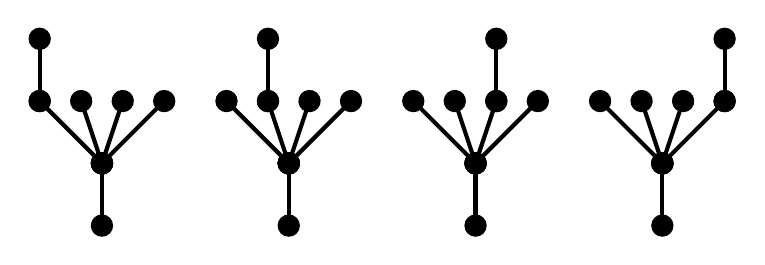
\begin{tikzpicture}[x=0.75pt,y=0.75pt,yscale=-1,xscale=1]
%uncomment if require: \path (0,300); %set diagram left start at 0, and has height of 300

%Straight Lines [id:da7271236022900844] 
\draw [line width=1.5]    (120,120) -- (90,90) ;
\draw [shift={(90,90)}, rotate = 225] [color={rgb, 255:red, 0; green, 0; blue, 0 }  ][fill={rgb, 255:red, 0; green, 0; blue, 0 }  ][line width=1.5]      (0, 0) circle [x radius= 4.36, y radius= 4.36]   ;
\draw [shift={(120,120)}, rotate = 225] [color={rgb, 255:red, 0; green, 0; blue, 0 }  ][fill={rgb, 255:red, 0; green, 0; blue, 0 }  ][line width=1.5]      (0, 0) circle [x radius= 4.36, y radius= 4.36]   ;
%Straight Lines [id:da8829298962249057] 
\draw [line width=1.5]    (120,120) -- (110,90) ;
\draw [shift={(110,90)}, rotate = 251.57] [color={rgb, 255:red, 0; green, 0; blue, 0 }  ][fill={rgb, 255:red, 0; green, 0; blue, 0 }  ][line width=1.5]      (0, 0) circle [x radius= 4.36, y radius= 4.36]   ;
\draw [shift={(120,120)}, rotate = 251.57] [color={rgb, 255:red, 0; green, 0; blue, 0 }  ][fill={rgb, 255:red, 0; green, 0; blue, 0 }  ][line width=1.5]      (0, 0) circle [x radius= 4.36, y radius= 4.36]   ;
%Straight Lines [id:da14019661944022443] 
\draw [line width=1.5]    (120,120) -- (150,90) ;
\draw [shift={(150,90)}, rotate = 315] [color={rgb, 255:red, 0; green, 0; blue, 0 }  ][fill={rgb, 255:red, 0; green, 0; blue, 0 }  ][line width=1.5]      (0, 0) circle [x radius= 4.36, y radius= 4.36]   ;
\draw [shift={(120,120)}, rotate = 315] [color={rgb, 255:red, 0; green, 0; blue, 0 }  ][fill={rgb, 255:red, 0; green, 0; blue, 0 }  ][line width=1.5]      (0, 0) circle [x radius= 4.36, y radius= 4.36]   ;
%Straight Lines [id:da3561053996918748] 
\draw [line width=1.5]    (120,150) -- (120,120) ;
\draw [shift={(120,120)}, rotate = 270] [color={rgb, 255:red, 0; green, 0; blue, 0 }  ][fill={rgb, 255:red, 0; green, 0; blue, 0 }  ][line width=1.5]      (0, 0) circle [x radius= 4.36, y radius= 4.36]   ;
\draw [shift={(120,150)}, rotate = 270] [color={rgb, 255:red, 0; green, 0; blue, 0 }  ][fill={rgb, 255:red, 0; green, 0; blue, 0 }  ][line width=1.5]      (0, 0) circle [x radius= 4.36, y radius= 4.36]   ;
%Straight Lines [id:da12959305658190345] 
\draw [line width=1.5]    (130,90) -- (120,120) ;
\draw [shift={(120,120)}, rotate = 108.43] [color={rgb, 255:red, 0; green, 0; blue, 0 }  ][fill={rgb, 255:red, 0; green, 0; blue, 0 }  ][line width=1.5]      (0, 0) circle [x radius= 4.36, y radius= 4.36]   ;
\draw [shift={(130,90)}, rotate = 108.43] [color={rgb, 255:red, 0; green, 0; blue, 0 }  ][fill={rgb, 255:red, 0; green, 0; blue, 0 }  ][line width=1.5]      (0, 0) circle [x radius= 4.36, y radius= 4.36]   ;
%Straight Lines [id:da17788889705056876] 
\draw [line width=1.5]    (210,120) -- (180,90) ;
\draw [shift={(180,90)}, rotate = 225] [color={rgb, 255:red, 0; green, 0; blue, 0 }  ][fill={rgb, 255:red, 0; green, 0; blue, 0 }  ][line width=1.5]      (0, 0) circle [x radius= 4.36, y radius= 4.36]   ;
\draw [shift={(210,120)}, rotate = 225] [color={rgb, 255:red, 0; green, 0; blue, 0 }  ][fill={rgb, 255:red, 0; green, 0; blue, 0 }  ][line width=1.5]      (0, 0) circle [x radius= 4.36, y radius= 4.36]   ;
%Straight Lines [id:da32726690992182617] 
\draw [line width=1.5]    (210,120) -- (200,90) ;
\draw [shift={(200,90)}, rotate = 251.57] [color={rgb, 255:red, 0; green, 0; blue, 0 }  ][fill={rgb, 255:red, 0; green, 0; blue, 0 }  ][line width=1.5]      (0, 0) circle [x radius= 4.36, y radius= 4.36]   ;
\draw [shift={(210,120)}, rotate = 251.57] [color={rgb, 255:red, 0; green, 0; blue, 0 }  ][fill={rgb, 255:red, 0; green, 0; blue, 0 }  ][line width=1.5]      (0, 0) circle [x radius= 4.36, y radius= 4.36]   ;
%Straight Lines [id:da6529521762459134] 
\draw [line width=1.5]    (210,120) -- (240,90) ;
\draw [shift={(240,90)}, rotate = 315] [color={rgb, 255:red, 0; green, 0; blue, 0 }  ][fill={rgb, 255:red, 0; green, 0; blue, 0 }  ][line width=1.5]      (0, 0) circle [x radius= 4.36, y radius= 4.36]   ;
\draw [shift={(210,120)}, rotate = 315] [color={rgb, 255:red, 0; green, 0; blue, 0 }  ][fill={rgb, 255:red, 0; green, 0; blue, 0 }  ][line width=1.5]      (0, 0) circle [x radius= 4.36, y radius= 4.36]   ;
%Straight Lines [id:da10508941767197344] 
\draw [line width=1.5]    (210,150) -- (210,120) ;
\draw [shift={(210,120)}, rotate = 270] [color={rgb, 255:red, 0; green, 0; blue, 0 }  ][fill={rgb, 255:red, 0; green, 0; blue, 0 }  ][line width=1.5]      (0, 0) circle [x radius= 4.36, y radius= 4.36]   ;
\draw [shift={(210,150)}, rotate = 270] [color={rgb, 255:red, 0; green, 0; blue, 0 }  ][fill={rgb, 255:red, 0; green, 0; blue, 0 }  ][line width=1.5]      (0, 0) circle [x radius= 4.36, y radius= 4.36]   ;
%Straight Lines [id:da6259633442377939] 
\draw [line width=1.5]    (220,90) -- (210,120) ;
\draw [shift={(210,120)}, rotate = 108.43] [color={rgb, 255:red, 0; green, 0; blue, 0 }  ][fill={rgb, 255:red, 0; green, 0; blue, 0 }  ][line width=1.5]      (0, 0) circle [x radius= 4.36, y radius= 4.36]   ;
\draw [shift={(220,90)}, rotate = 108.43] [color={rgb, 255:red, 0; green, 0; blue, 0 }  ][fill={rgb, 255:red, 0; green, 0; blue, 0 }  ][line width=1.5]      (0, 0) circle [x radius= 4.36, y radius= 4.36]   ;
%Straight Lines [id:da18827403823128308] 
\draw [line width=1.5]    (300,120) -- (270,90) ;
\draw [shift={(270,90)}, rotate = 225] [color={rgb, 255:red, 0; green, 0; blue, 0 }  ][fill={rgb, 255:red, 0; green, 0; blue, 0 }  ][line width=1.5]      (0, 0) circle [x radius= 4.36, y radius= 4.36]   ;
\draw [shift={(300,120)}, rotate = 225] [color={rgb, 255:red, 0; green, 0; blue, 0 }  ][fill={rgb, 255:red, 0; green, 0; blue, 0 }  ][line width=1.5]      (0, 0) circle [x radius= 4.36, y radius= 4.36]   ;
%Straight Lines [id:da4416224263321782] 
\draw [line width=1.5]    (300,120) -- (290,90) ;
\draw [shift={(290,90)}, rotate = 251.57] [color={rgb, 255:red, 0; green, 0; blue, 0 }  ][fill={rgb, 255:red, 0; green, 0; blue, 0 }  ][line width=1.5]      (0, 0) circle [x radius= 4.36, y radius= 4.36]   ;
\draw [shift={(300,120)}, rotate = 251.57] [color={rgb, 255:red, 0; green, 0; blue, 0 }  ][fill={rgb, 255:red, 0; green, 0; blue, 0 }  ][line width=1.5]      (0, 0) circle [x radius= 4.36, y radius= 4.36]   ;
%Straight Lines [id:da4912193105487581] 
\draw [line width=1.5]    (300,120) -- (330,90) ;
\draw [shift={(330,90)}, rotate = 315] [color={rgb, 255:red, 0; green, 0; blue, 0 }  ][fill={rgb, 255:red, 0; green, 0; blue, 0 }  ][line width=1.5]      (0, 0) circle [x radius= 4.36, y radius= 4.36]   ;
\draw [shift={(300,120)}, rotate = 315] [color={rgb, 255:red, 0; green, 0; blue, 0 }  ][fill={rgb, 255:red, 0; green, 0; blue, 0 }  ][line width=1.5]      (0, 0) circle [x radius= 4.36, y radius= 4.36]   ;
%Straight Lines [id:da057140828311111225] 
\draw [line width=1.5]    (300,150) -- (300,120) ;
\draw [shift={(300,120)}, rotate = 270] [color={rgb, 255:red, 0; green, 0; blue, 0 }  ][fill={rgb, 255:red, 0; green, 0; blue, 0 }  ][line width=1.5]      (0, 0) circle [x radius= 4.36, y radius= 4.36]   ;
\draw [shift={(300,150)}, rotate = 270] [color={rgb, 255:red, 0; green, 0; blue, 0 }  ][fill={rgb, 255:red, 0; green, 0; blue, 0 }  ][line width=1.5]      (0, 0) circle [x radius= 4.36, y radius= 4.36]   ;
%Straight Lines [id:da6532175337656438] 
\draw [line width=1.5]    (310,90) -- (300,120) ;
\draw [shift={(300,120)}, rotate = 108.43] [color={rgb, 255:red, 0; green, 0; blue, 0 }  ][fill={rgb, 255:red, 0; green, 0; blue, 0 }  ][line width=1.5]      (0, 0) circle [x radius= 4.36, y radius= 4.36]   ;
\draw [shift={(310,90)}, rotate = 108.43] [color={rgb, 255:red, 0; green, 0; blue, 0 }  ][fill={rgb, 255:red, 0; green, 0; blue, 0 }  ][line width=1.5]      (0, 0) circle [x radius= 4.36, y radius= 4.36]   ;
%Straight Lines [id:da9439423309856876] 
\draw [line width=1.5]    (390,120) -- (360,90) ;
\draw [shift={(360,90)}, rotate = 225] [color={rgb, 255:red, 0; green, 0; blue, 0 }  ][fill={rgb, 255:red, 0; green, 0; blue, 0 }  ][line width=1.5]      (0, 0) circle [x radius= 4.36, y radius= 4.36]   ;
\draw [shift={(390,120)}, rotate = 225] [color={rgb, 255:red, 0; green, 0; blue, 0 }  ][fill={rgb, 255:red, 0; green, 0; blue, 0 }  ][line width=1.5]      (0, 0) circle [x radius= 4.36, y radius= 4.36]   ;
%Straight Lines [id:da6793777254659024] 
\draw [line width=1.5]    (390,120) -- (380,90) ;
\draw [shift={(380,90)}, rotate = 251.57] [color={rgb, 255:red, 0; green, 0; blue, 0 }  ][fill={rgb, 255:red, 0; green, 0; blue, 0 }  ][line width=1.5]      (0, 0) circle [x radius= 4.36, y radius= 4.36]   ;
\draw [shift={(390,120)}, rotate = 251.57] [color={rgb, 255:red, 0; green, 0; blue, 0 }  ][fill={rgb, 255:red, 0; green, 0; blue, 0 }  ][line width=1.5]      (0, 0) circle [x radius= 4.36, y radius= 4.36]   ;
%Straight Lines [id:da4673813785992058] 
\draw [line width=1.5]    (390,120) -- (420,90) ;
\draw [shift={(420,90)}, rotate = 315] [color={rgb, 255:red, 0; green, 0; blue, 0 }  ][fill={rgb, 255:red, 0; green, 0; blue, 0 }  ][line width=1.5]      (0, 0) circle [x radius= 4.36, y radius= 4.36]   ;
\draw [shift={(390,120)}, rotate = 315] [color={rgb, 255:red, 0; green, 0; blue, 0 }  ][fill={rgb, 255:red, 0; green, 0; blue, 0 }  ][line width=1.5]      (0, 0) circle [x radius= 4.36, y radius= 4.36]   ;
%Straight Lines [id:da2972746595471605] 
\draw [line width=1.5]    (390,150) -- (390,120) ;
\draw [shift={(390,120)}, rotate = 270] [color={rgb, 255:red, 0; green, 0; blue, 0 }  ][fill={rgb, 255:red, 0; green, 0; blue, 0 }  ][line width=1.5]      (0, 0) circle [x radius= 4.36, y radius= 4.36]   ;
\draw [shift={(390,150)}, rotate = 270] [color={rgb, 255:red, 0; green, 0; blue, 0 }  ][fill={rgb, 255:red, 0; green, 0; blue, 0 }  ][line width=1.5]      (0, 0) circle [x radius= 4.36, y radius= 4.36]   ;
%Straight Lines [id:da526738135792] 
\draw [line width=1.5]    (400,90) -- (390,120) ;
\draw [shift={(390,120)}, rotate = 108.43] [color={rgb, 255:red, 0; green, 0; blue, 0 }  ][fill={rgb, 255:red, 0; green, 0; blue, 0 }  ][line width=1.5]      (0, 0) circle [x radius= 4.36, y radius= 4.36]   ;
\draw [shift={(400,90)}, rotate = 108.43] [color={rgb, 255:red, 0; green, 0; blue, 0 }  ][fill={rgb, 255:red, 0; green, 0; blue, 0 }  ][line width=1.5]      (0, 0) circle [x radius= 4.36, y radius= 4.36]   ;
%Straight Lines [id:da3439286430792807] 
\draw [line width=1.5]    (90,90) -- (90,60) ;
\draw [shift={(90,60)}, rotate = 270] [color={rgb, 255:red, 0; green, 0; blue, 0 }  ][fill={rgb, 255:red, 0; green, 0; blue, 0 }  ][line width=1.5]      (0, 0) circle [x radius= 4.36, y radius= 4.36]   ;
\draw [shift={(90,90)}, rotate = 270] [color={rgb, 255:red, 0; green, 0; blue, 0 }  ][fill={rgb, 255:red, 0; green, 0; blue, 0 }  ][line width=1.5]      (0, 0) circle [x radius= 4.36, y radius= 4.36]   ;
%Straight Lines [id:da027749002350105467] 
\draw [line width=1.5]    (200,90) -- (200,60) ;
\draw [shift={(200,60)}, rotate = 270] [color={rgb, 255:red, 0; green, 0; blue, 0 }  ][fill={rgb, 255:red, 0; green, 0; blue, 0 }  ][line width=1.5]      (0, 0) circle [x radius= 4.36, y radius= 4.36]   ;
\draw [shift={(200,90)}, rotate = 270] [color={rgb, 255:red, 0; green, 0; blue, 0 }  ][fill={rgb, 255:red, 0; green, 0; blue, 0 }  ][line width=1.5]      (0, 0) circle [x radius= 4.36, y radius= 4.36]   ;
%Straight Lines [id:da4141601555763963] 
\draw [line width=1.5]    (310,90) -- (310,60) ;
\draw [shift={(310,60)}, rotate = 270] [color={rgb, 255:red, 0; green, 0; blue, 0 }  ][fill={rgb, 255:red, 0; green, 0; blue, 0 }  ][line width=1.5]      (0, 0) circle [x radius= 4.36, y radius= 4.36]   ;
\draw [shift={(310,90)}, rotate = 270] [color={rgb, 255:red, 0; green, 0; blue, 0 }  ][fill={rgb, 255:red, 0; green, 0; blue, 0 }  ][line width=1.5]      (0, 0) circle [x radius= 4.36, y radius= 4.36]   ;
%Straight Lines [id:da8143971343614638] 
\draw [line width=1.5]    (420,90) -- (420,60) ;
\draw [shift={(420,60)}, rotate = 270] [color={rgb, 255:red, 0; green, 0; blue, 0 }  ][fill={rgb, 255:red, 0; green, 0; blue, 0 }  ][line width=1.5]      (0, 0) circle [x radius= 4.36, y radius= 4.36]   ;
\draw [shift={(420,90)}, rotate = 270] [color={rgb, 255:red, 0; green, 0; blue, 0 }  ][fill={rgb, 255:red, 0; green, 0; blue, 0 }  ][line width=1.5]      (0, 0) circle [x radius= 4.36, y radius= 4.36]   ;
\end{tikzpicture}
\end{center}

\begin{enumerate}
\setcounter{enumi}{2}
    \item If $n$ is odd, put positive signs, $+$, between them all, and if $n$ is even put negative signs, $-$. 
    \item Then draw $n-1$ copies of the binary rooted tree that represent $m_{n-1}$ below the above trees. \item Put a copy of $m_2$ on the leaves in the same way as we did for $m_1$ on $m_n$.
    \item Put alternating signs, beginning with $+$ between the different trees.
\end{enumerate}

In the $n=4$ example we drew above, we would get

% Example of the two first rows of the correct sign procedure for n=4



\begin{center}
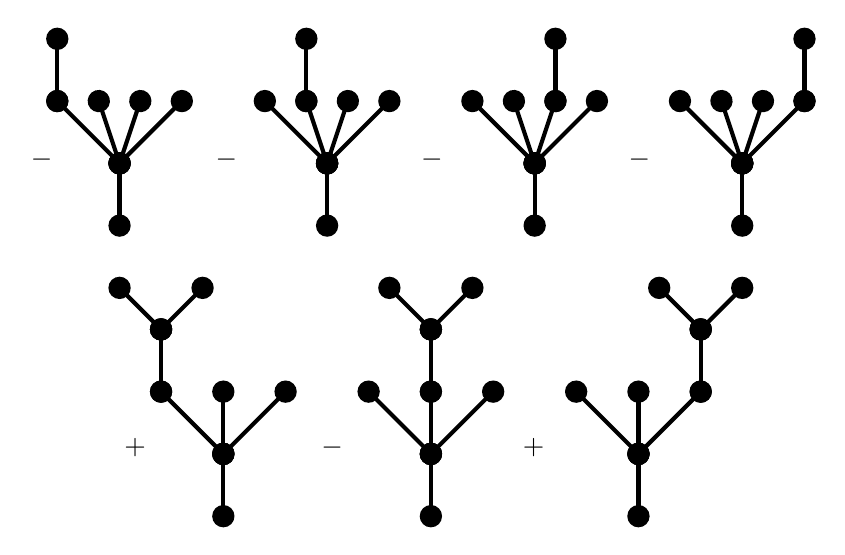
\begin{tikzpicture}[x=0.75pt,y=0.75pt,yscale=-1,xscale=1]
%uncomment if require: \path (0,300); %set diagram left start at 0, and has height of 300

%Straight Lines [id:da7271236022900844] 
\draw [line width=1.5]    (50,70) -- (20,40) ;
\draw [shift={(20,40)}, rotate = 225] [color={rgb, 255:red, 0; green, 0; blue, 0 }  ][fill={rgb, 255:red, 0; green, 0; blue, 0 }  ][line width=1.5]      (0, 0) circle [x radius= 4.36, y radius= 4.36]   ;
\draw [shift={(50,70)}, rotate = 225] [color={rgb, 255:red, 0; green, 0; blue, 0 }  ][fill={rgb, 255:red, 0; green, 0; blue, 0 }  ][line width=1.5]      (0, 0) circle [x radius= 4.36, y radius= 4.36]   ;
%Straight Lines [id:da8829298962249057] 
\draw [line width=1.5]    (50,70) -- (40,40) ;
\draw [shift={(40,40)}, rotate = 251.57] [color={rgb, 255:red, 0; green, 0; blue, 0 }  ][fill={rgb, 255:red, 0; green, 0; blue, 0 }  ][line width=1.5]      (0, 0) circle [x radius= 4.36, y radius= 4.36]   ;
\draw [shift={(50,70)}, rotate = 251.57] [color={rgb, 255:red, 0; green, 0; blue, 0 }  ][fill={rgb, 255:red, 0; green, 0; blue, 0 }  ][line width=1.5]      (0, 0) circle [x radius= 4.36, y radius= 4.36]   ;
%Straight Lines [id:da14019661944022443] 
\draw [line width=1.5]    (50,70) -- (80,40) ;
\draw [shift={(80,40)}, rotate = 315] [color={rgb, 255:red, 0; green, 0; blue, 0 }  ][fill={rgb, 255:red, 0; green, 0; blue, 0 }  ][line width=1.5]      (0, 0) circle [x radius= 4.36, y radius= 4.36]   ;
\draw [shift={(50,70)}, rotate = 315] [color={rgb, 255:red, 0; green, 0; blue, 0 }  ][fill={rgb, 255:red, 0; green, 0; blue, 0 }  ][line width=1.5]      (0, 0) circle [x radius= 4.36, y radius= 4.36]   ;
%Straight Lines [id:da3561053996918748] 
\draw [line width=1.5]    (50,100) -- (50,70) ;
\draw [shift={(50,70)}, rotate = 270] [color={rgb, 255:red, 0; green, 0; blue, 0 }  ][fill={rgb, 255:red, 0; green, 0; blue, 0 }  ][line width=1.5]      (0, 0) circle [x radius= 4.36, y radius= 4.36]   ;
\draw [shift={(50,100)}, rotate = 270] [color={rgb, 255:red, 0; green, 0; blue, 0 }  ][fill={rgb, 255:red, 0; green, 0; blue, 0 }  ][line width=1.5]      (0, 0) circle [x radius= 4.36, y radius= 4.36]   ;
%Straight Lines [id:da12959305658190345] 
\draw [line width=1.5]    (60,40) -- (50,70) ;
\draw [shift={(50,70)}, rotate = 108.43] [color={rgb, 255:red, 0; green, 0; blue, 0 }  ][fill={rgb, 255:red, 0; green, 0; blue, 0 }  ][line width=1.5]      (0, 0) circle [x radius= 4.36, y radius= 4.36]   ;
\draw [shift={(60,40)}, rotate = 108.43] [color={rgb, 255:red, 0; green, 0; blue, 0 }  ][fill={rgb, 255:red, 0; green, 0; blue, 0 }  ][line width=1.5]      (0, 0) circle [x radius= 4.36, y radius= 4.36]   ;
%Straight Lines [id:da17788889705056876] 
\draw [line width=1.5]    (150,70) -- (120,40) ;
\draw [shift={(120,40)}, rotate = 225] [color={rgb, 255:red, 0; green, 0; blue, 0 }  ][fill={rgb, 255:red, 0; green, 0; blue, 0 }  ][line width=1.5]      (0, 0) circle [x radius= 4.36, y radius= 4.36]   ;
\draw [shift={(150,70)}, rotate = 225] [color={rgb, 255:red, 0; green, 0; blue, 0 }  ][fill={rgb, 255:red, 0; green, 0; blue, 0 }  ][line width=1.5]      (0, 0) circle [x radius= 4.36, y radius= 4.36]   ;
%Straight Lines [id:da32726690992182617] 
\draw [line width=1.5]    (150,70) -- (140,40) ;
\draw [shift={(140,40)}, rotate = 251.57] [color={rgb, 255:red, 0; green, 0; blue, 0 }  ][fill={rgb, 255:red, 0; green, 0; blue, 0 }  ][line width=1.5]      (0, 0) circle [x radius= 4.36, y radius= 4.36]   ;
\draw [shift={(150,70)}, rotate = 251.57] [color={rgb, 255:red, 0; green, 0; blue, 0 }  ][fill={rgb, 255:red, 0; green, 0; blue, 0 }  ][line width=1.5]      (0, 0) circle [x radius= 4.36, y radius= 4.36]   ;
%Straight Lines [id:da6529521762459134] 
\draw [line width=1.5]    (150,70) -- (180,40) ;
\draw [shift={(180,40)}, rotate = 315] [color={rgb, 255:red, 0; green, 0; blue, 0 }  ][fill={rgb, 255:red, 0; green, 0; blue, 0 }  ][line width=1.5]      (0, 0) circle [x radius= 4.36, y radius= 4.36]   ;
\draw [shift={(150,70)}, rotate = 315] [color={rgb, 255:red, 0; green, 0; blue, 0 }  ][fill={rgb, 255:red, 0; green, 0; blue, 0 }  ][line width=1.5]      (0, 0) circle [x radius= 4.36, y radius= 4.36]   ;
%Straight Lines [id:da10508941767197344] 
\draw [line width=1.5]    (150,100) -- (150,70) ;
\draw [shift={(150,70)}, rotate = 270] [color={rgb, 255:red, 0; green, 0; blue, 0 }  ][fill={rgb, 255:red, 0; green, 0; blue, 0 }  ][line width=1.5]      (0, 0) circle [x radius= 4.36, y radius= 4.36]   ;
\draw [shift={(150,100)}, rotate = 270] [color={rgb, 255:red, 0; green, 0; blue, 0 }  ][fill={rgb, 255:red, 0; green, 0; blue, 0 }  ][line width=1.5]      (0, 0) circle [x radius= 4.36, y radius= 4.36]   ;
%Straight Lines [id:da6259633442377939] 
\draw [line width=1.5]    (160,40) -- (150,70) ;
\draw [shift={(150,70)}, rotate = 108.43] [color={rgb, 255:red, 0; green, 0; blue, 0 }  ][fill={rgb, 255:red, 0; green, 0; blue, 0 }  ][line width=1.5]      (0, 0) circle [x radius= 4.36, y radius= 4.36]   ;
\draw [shift={(160,40)}, rotate = 108.43] [color={rgb, 255:red, 0; green, 0; blue, 0 }  ][fill={rgb, 255:red, 0; green, 0; blue, 0 }  ][line width=1.5]      (0, 0) circle [x radius= 4.36, y radius= 4.36]   ;
%Straight Lines [id:da18827403823128308] 
\draw [line width=1.5]    (250,70) -- (220,40) ;
\draw [shift={(220,40)}, rotate = 225] [color={rgb, 255:red, 0; green, 0; blue, 0 }  ][fill={rgb, 255:red, 0; green, 0; blue, 0 }  ][line width=1.5]      (0, 0) circle [x radius= 4.36, y radius= 4.36]   ;
\draw [shift={(250,70)}, rotate = 225] [color={rgb, 255:red, 0; green, 0; blue, 0 }  ][fill={rgb, 255:red, 0; green, 0; blue, 0 }  ][line width=1.5]      (0, 0) circle [x radius= 4.36, y radius= 4.36]   ;
%Straight Lines [id:da4416224263321782] 
\draw [line width=1.5]    (250,70) -- (240,40) ;
\draw [shift={(240,40)}, rotate = 251.57] [color={rgb, 255:red, 0; green, 0; blue, 0 }  ][fill={rgb, 255:red, 0; green, 0; blue, 0 }  ][line width=1.5]      (0, 0) circle [x radius= 4.36, y radius= 4.36]   ;
\draw [shift={(250,70)}, rotate = 251.57] [color={rgb, 255:red, 0; green, 0; blue, 0 }  ][fill={rgb, 255:red, 0; green, 0; blue, 0 }  ][line width=1.5]      (0, 0) circle [x radius= 4.36, y radius= 4.36]   ;
%Straight Lines [id:da4912193105487581] 
\draw [line width=1.5]    (250,70) -- (280,40) ;
\draw [shift={(280,40)}, rotate = 315] [color={rgb, 255:red, 0; green, 0; blue, 0 }  ][fill={rgb, 255:red, 0; green, 0; blue, 0 }  ][line width=1.5]      (0, 0) circle [x radius= 4.36, y radius= 4.36]   ;
\draw [shift={(250,70)}, rotate = 315] [color={rgb, 255:red, 0; green, 0; blue, 0 }  ][fill={rgb, 255:red, 0; green, 0; blue, 0 }  ][line width=1.5]      (0, 0) circle [x radius= 4.36, y radius= 4.36]   ;
%Straight Lines [id:da057140828311111225] 
\draw [line width=1.5]    (250,100) -- (250,70) ;
\draw [shift={(250,70)}, rotate = 270] [color={rgb, 255:red, 0; green, 0; blue, 0 }  ][fill={rgb, 255:red, 0; green, 0; blue, 0 }  ][line width=1.5]      (0, 0) circle [x radius= 4.36, y radius= 4.36]   ;
\draw [shift={(250,100)}, rotate = 270] [color={rgb, 255:red, 0; green, 0; blue, 0 }  ][fill={rgb, 255:red, 0; green, 0; blue, 0 }  ][line width=1.5]      (0, 0) circle [x radius= 4.36, y radius= 4.36]   ;
%Straight Lines [id:da6532175337656438] 
\draw [line width=1.5]    (260,40) -- (250,70) ;
\draw [shift={(250,70)}, rotate = 108.43] [color={rgb, 255:red, 0; green, 0; blue, 0 }  ][fill={rgb, 255:red, 0; green, 0; blue, 0 }  ][line width=1.5]      (0, 0) circle [x radius= 4.36, y radius= 4.36]   ;
\draw [shift={(260,40)}, rotate = 108.43] [color={rgb, 255:red, 0; green, 0; blue, 0 }  ][fill={rgb, 255:red, 0; green, 0; blue, 0 }  ][line width=1.5]      (0, 0) circle [x radius= 4.36, y radius= 4.36]   ;
%Straight Lines [id:da9439423309856876] 
\draw [line width=1.5]    (350,70) -- (320,40) ;
\draw [shift={(320,40)}, rotate = 225] [color={rgb, 255:red, 0; green, 0; blue, 0 }  ][fill={rgb, 255:red, 0; green, 0; blue, 0 }  ][line width=1.5]      (0, 0) circle [x radius= 4.36, y radius= 4.36]   ;
\draw [shift={(350,70)}, rotate = 225] [color={rgb, 255:red, 0; green, 0; blue, 0 }  ][fill={rgb, 255:red, 0; green, 0; blue, 0 }  ][line width=1.5]      (0, 0) circle [x radius= 4.36, y radius= 4.36]   ;
%Straight Lines [id:da6793777254659024] 
\draw [line width=1.5]    (350,70) -- (340,40) ;
\draw [shift={(340,40)}, rotate = 251.57] [color={rgb, 255:red, 0; green, 0; blue, 0 }  ][fill={rgb, 255:red, 0; green, 0; blue, 0 }  ][line width=1.5]      (0, 0) circle [x radius= 4.36, y radius= 4.36]   ;
\draw [shift={(350,70)}, rotate = 251.57] [color={rgb, 255:red, 0; green, 0; blue, 0 }  ][fill={rgb, 255:red, 0; green, 0; blue, 0 }  ][line width=1.5]      (0, 0) circle [x radius= 4.36, y radius= 4.36]   ;
%Straight Lines [id:da4673813785992058] 
\draw [line width=1.5]    (350,70) -- (380,40) ;
\draw [shift={(380,40)}, rotate = 315] [color={rgb, 255:red, 0; green, 0; blue, 0 }  ][fill={rgb, 255:red, 0; green, 0; blue, 0 }  ][line width=1.5]      (0, 0) circle [x radius= 4.36, y radius= 4.36]   ;
\draw [shift={(350,70)}, rotate = 315] [color={rgb, 255:red, 0; green, 0; blue, 0 }  ][fill={rgb, 255:red, 0; green, 0; blue, 0 }  ][line width=1.5]      (0, 0) circle [x radius= 4.36, y radius= 4.36]   ;
%Straight Lines [id:da2972746595471605] 
\draw [line width=1.5]    (350,100) -- (350,70) ;
\draw [shift={(350,70)}, rotate = 270] [color={rgb, 255:red, 0; green, 0; blue, 0 }  ][fill={rgb, 255:red, 0; green, 0; blue, 0 }  ][line width=1.5]      (0, 0) circle [x radius= 4.36, y radius= 4.36]   ;
\draw [shift={(350,100)}, rotate = 270] [color={rgb, 255:red, 0; green, 0; blue, 0 }  ][fill={rgb, 255:red, 0; green, 0; blue, 0 }  ][line width=1.5]      (0, 0) circle [x radius= 4.36, y radius= 4.36]   ;
%Straight Lines [id:da526738135792] 
\draw [line width=1.5]    (360,40) -- (350,70) ;
\draw [shift={(350,70)}, rotate = 108.43] [color={rgb, 255:red, 0; green, 0; blue, 0 }  ][fill={rgb, 255:red, 0; green, 0; blue, 0 }  ][line width=1.5]      (0, 0) circle [x radius= 4.36, y radius= 4.36]   ;
\draw [shift={(360,40)}, rotate = 108.43] [color={rgb, 255:red, 0; green, 0; blue, 0 }  ][fill={rgb, 255:red, 0; green, 0; blue, 0 }  ][line width=1.5]      (0, 0) circle [x radius= 4.36, y radius= 4.36]   ;
%Straight Lines [id:da3439286430792807] 
\draw [line width=1.5]    (20,40) -- (20,10) ;
\draw [shift={(20,10)}, rotate = 270] [color={rgb, 255:red, 0; green, 0; blue, 0 }  ][fill={rgb, 255:red, 0; green, 0; blue, 0 }  ][line width=1.5]      (0, 0) circle [x radius= 4.36, y radius= 4.36]   ;
\draw [shift={(20,40)}, rotate = 270] [color={rgb, 255:red, 0; green, 0; blue, 0 }  ][fill={rgb, 255:red, 0; green, 0; blue, 0 }  ][line width=1.5]      (0, 0) circle [x radius= 4.36, y radius= 4.36]   ;
%Straight Lines [id:da027749002350105467] 
\draw [line width=1.5]    (140,40) -- (140,10) ;
\draw [shift={(140,10)}, rotate = 270] [color={rgb, 255:red, 0; green, 0; blue, 0 }  ][fill={rgb, 255:red, 0; green, 0; blue, 0 }  ][line width=1.5]      (0, 0) circle [x radius= 4.36, y radius= 4.36]   ;
\draw [shift={(140,40)}, rotate = 270] [color={rgb, 255:red, 0; green, 0; blue, 0 }  ][fill={rgb, 255:red, 0; green, 0; blue, 0 }  ][line width=1.5]      (0, 0) circle [x radius= 4.36, y radius= 4.36]   ;
%Straight Lines [id:da4141601555763963] 
\draw [line width=1.5]    (260,40) -- (260,10) ;
\draw [shift={(260,10)}, rotate = 270] [color={rgb, 255:red, 0; green, 0; blue, 0 }  ][fill={rgb, 255:red, 0; green, 0; blue, 0 }  ][line width=1.5]      (0, 0) circle [x radius= 4.36, y radius= 4.36]   ;
\draw [shift={(260,40)}, rotate = 270] [color={rgb, 255:red, 0; green, 0; blue, 0 }  ][fill={rgb, 255:red, 0; green, 0; blue, 0 }  ][line width=1.5]      (0, 0) circle [x radius= 4.36, y radius= 4.36]   ;
%Straight Lines [id:da8143971343614638] 
\draw [line width=1.5]    (380,40) -- (380,10) ;
\draw [shift={(380,10)}, rotate = 270] [color={rgb, 255:red, 0; green, 0; blue, 0 }  ][fill={rgb, 255:red, 0; green, 0; blue, 0 }  ][line width=1.5]      (0, 0) circle [x radius= 4.36, y radius= 4.36]   ;
\draw [shift={(380,40)}, rotate = 270] [color={rgb, 255:red, 0; green, 0; blue, 0 }  ][fill={rgb, 255:red, 0; green, 0; blue, 0 }  ][line width=1.5]      (0, 0) circle [x radius= 4.36, y radius= 4.36]   ;
%Straight Lines [id:da5027840919946027] 
\draw [line width=1.5]    (100,210) -- (70,180) ;
\draw [shift={(70,180)}, rotate = 225] [color={rgb, 255:red, 0; green, 0; blue, 0 }  ][fill={rgb, 255:red, 0; green, 0; blue, 0 }  ][line width=1.5]      (0, 0) circle [x radius= 4.36, y radius= 4.36]   ;
\draw [shift={(100,210)}, rotate = 225] [color={rgb, 255:red, 0; green, 0; blue, 0 }  ][fill={rgb, 255:red, 0; green, 0; blue, 0 }  ][line width=1.5]      (0, 0) circle [x radius= 4.36, y radius= 4.36]   ;
%Straight Lines [id:da012169408330350517] 
\draw [line width=1.5]    (100,210) -- (100,180) ;
\draw [shift={(100,180)}, rotate = 270] [color={rgb, 255:red, 0; green, 0; blue, 0 }  ][fill={rgb, 255:red, 0; green, 0; blue, 0 }  ][line width=1.5]      (0, 0) circle [x radius= 4.36, y radius= 4.36]   ;
\draw [shift={(100,210)}, rotate = 270] [color={rgb, 255:red, 0; green, 0; blue, 0 }  ][fill={rgb, 255:red, 0; green, 0; blue, 0 }  ][line width=1.5]      (0, 0) circle [x radius= 4.36, y radius= 4.36]   ;
%Straight Lines [id:da3794956070144304] 
\draw [line width=1.5]    (100,210) -- (130,180) ;
\draw [shift={(130,180)}, rotate = 315] [color={rgb, 255:red, 0; green, 0; blue, 0 }  ][fill={rgb, 255:red, 0; green, 0; blue, 0 }  ][line width=1.5]      (0, 0) circle [x radius= 4.36, y radius= 4.36]   ;
\draw [shift={(100,210)}, rotate = 315] [color={rgb, 255:red, 0; green, 0; blue, 0 }  ][fill={rgb, 255:red, 0; green, 0; blue, 0 }  ][line width=1.5]      (0, 0) circle [x radius= 4.36, y radius= 4.36]   ;
%Straight Lines [id:da8996197602070666] 
\draw [line width=1.5]    (100,240) -- (100,210) ;
\draw [shift={(100,210)}, rotate = 270] [color={rgb, 255:red, 0; green, 0; blue, 0 }  ][fill={rgb, 255:red, 0; green, 0; blue, 0 }  ][line width=1.5]      (0, 0) circle [x radius= 4.36, y radius= 4.36]   ;
\draw [shift={(100,240)}, rotate = 270] [color={rgb, 255:red, 0; green, 0; blue, 0 }  ][fill={rgb, 255:red, 0; green, 0; blue, 0 }  ][line width=1.5]      (0, 0) circle [x radius= 4.36, y radius= 4.36]   ;
%Straight Lines [id:da1531842966441921] 
\draw [line width=1.5]    (70,150) -- (50,130) ;
\draw [shift={(50,130)}, rotate = 225] [color={rgb, 255:red, 0; green, 0; blue, 0 }  ][fill={rgb, 255:red, 0; green, 0; blue, 0 }  ][line width=1.5]      (0, 0) circle [x radius= 4.36, y radius= 4.36]   ;
\draw [shift={(70,150)}, rotate = 225] [color={rgb, 255:red, 0; green, 0; blue, 0 }  ][fill={rgb, 255:red, 0; green, 0; blue, 0 }  ][line width=1.5]      (0, 0) circle [x radius= 4.36, y radius= 4.36]   ;
%Straight Lines [id:da5635603151723407] 
\draw [line width=1.5]    (70,150) -- (90,130) ;
\draw [shift={(90,130)}, rotate = 315] [color={rgb, 255:red, 0; green, 0; blue, 0 }  ][fill={rgb, 255:red, 0; green, 0; blue, 0 }  ][line width=1.5]      (0, 0) circle [x radius= 4.36, y radius= 4.36]   ;
\draw [shift={(70,150)}, rotate = 315] [color={rgb, 255:red, 0; green, 0; blue, 0 }  ][fill={rgb, 255:red, 0; green, 0; blue, 0 }  ][line width=1.5]      (0, 0) circle [x radius= 4.36, y radius= 4.36]   ;
%Straight Lines [id:da37599967010410107] 
\draw [line width=1.5]    (70,180) -- (70,150) ;
\draw [shift={(70,150)}, rotate = 270] [color={rgb, 255:red, 0; green, 0; blue, 0 }  ][fill={rgb, 255:red, 0; green, 0; blue, 0 }  ][line width=1.5]      (0, 0) circle [x radius= 4.36, y radius= 4.36]   ;
\draw [shift={(70,180)}, rotate = 270] [color={rgb, 255:red, 0; green, 0; blue, 0 }  ][fill={rgb, 255:red, 0; green, 0; blue, 0 }  ][line width=1.5]      (0, 0) circle [x radius= 4.36, y radius= 4.36]   ;
%Straight Lines [id:da698265177656928] 
\draw [line width=1.5]    (200,210) -- (170,180) ;
\draw [shift={(170,180)}, rotate = 225] [color={rgb, 255:red, 0; green, 0; blue, 0 }  ][fill={rgb, 255:red, 0; green, 0; blue, 0 }  ][line width=1.5]      (0, 0) circle [x radius= 4.36, y radius= 4.36]   ;
\draw [shift={(200,210)}, rotate = 225] [color={rgb, 255:red, 0; green, 0; blue, 0 }  ][fill={rgb, 255:red, 0; green, 0; blue, 0 }  ][line width=1.5]      (0, 0) circle [x radius= 4.36, y radius= 4.36]   ;
%Straight Lines [id:da049456703112388256] 
\draw [line width=1.5]    (200,210) -- (200,180) ;
\draw [shift={(200,180)}, rotate = 270] [color={rgb, 255:red, 0; green, 0; blue, 0 }  ][fill={rgb, 255:red, 0; green, 0; blue, 0 }  ][line width=1.5]      (0, 0) circle [x radius= 4.36, y radius= 4.36]   ;
\draw [shift={(200,210)}, rotate = 270] [color={rgb, 255:red, 0; green, 0; blue, 0 }  ][fill={rgb, 255:red, 0; green, 0; blue, 0 }  ][line width=1.5]      (0, 0) circle [x radius= 4.36, y radius= 4.36]   ;
%Straight Lines [id:da19781405329398405] 
\draw [line width=1.5]    (200,210) -- (230,180) ;
\draw [shift={(230,180)}, rotate = 315] [color={rgb, 255:red, 0; green, 0; blue, 0 }  ][fill={rgb, 255:red, 0; green, 0; blue, 0 }  ][line width=1.5]      (0, 0) circle [x radius= 4.36, y radius= 4.36]   ;
\draw [shift={(200,210)}, rotate = 315] [color={rgb, 255:red, 0; green, 0; blue, 0 }  ][fill={rgb, 255:red, 0; green, 0; blue, 0 }  ][line width=1.5]      (0, 0) circle [x radius= 4.36, y radius= 4.36]   ;
%Straight Lines [id:da9771660287757578] 
\draw [line width=1.5]    (200,240) -- (200,210) ;
\draw [shift={(200,210)}, rotate = 270] [color={rgb, 255:red, 0; green, 0; blue, 0 }  ][fill={rgb, 255:red, 0; green, 0; blue, 0 }  ][line width=1.5]      (0, 0) circle [x radius= 4.36, y radius= 4.36]   ;
\draw [shift={(200,240)}, rotate = 270] [color={rgb, 255:red, 0; green, 0; blue, 0 }  ][fill={rgb, 255:red, 0; green, 0; blue, 0 }  ][line width=1.5]      (0, 0) circle [x radius= 4.36, y radius= 4.36]   ;
%Straight Lines [id:da8050669462477833] 
\draw [line width=1.5]    (200,150) -- (180,130) ;
\draw [shift={(180,130)}, rotate = 225] [color={rgb, 255:red, 0; green, 0; blue, 0 }  ][fill={rgb, 255:red, 0; green, 0; blue, 0 }  ][line width=1.5]      (0, 0) circle [x radius= 4.36, y radius= 4.36]   ;
\draw [shift={(200,150)}, rotate = 225] [color={rgb, 255:red, 0; green, 0; blue, 0 }  ][fill={rgb, 255:red, 0; green, 0; blue, 0 }  ][line width=1.5]      (0, 0) circle [x radius= 4.36, y radius= 4.36]   ;
%Straight Lines [id:da4433467710630703] 
\draw [line width=1.5]    (200,150) -- (220,130) ;
\draw [shift={(220,130)}, rotate = 315] [color={rgb, 255:red, 0; green, 0; blue, 0 }  ][fill={rgb, 255:red, 0; green, 0; blue, 0 }  ][line width=1.5]      (0, 0) circle [x radius= 4.36, y radius= 4.36]   ;
\draw [shift={(200,150)}, rotate = 315] [color={rgb, 255:red, 0; green, 0; blue, 0 }  ][fill={rgb, 255:red, 0; green, 0; blue, 0 }  ][line width=1.5]      (0, 0) circle [x radius= 4.36, y radius= 4.36]   ;
%Straight Lines [id:da01581391478939298] 
\draw [line width=1.5]    (200,180) -- (200,150) ;
\draw [shift={(200,150)}, rotate = 270] [color={rgb, 255:red, 0; green, 0; blue, 0 }  ][fill={rgb, 255:red, 0; green, 0; blue, 0 }  ][line width=1.5]      (0, 0) circle [x radius= 4.36, y radius= 4.36]   ;
\draw [shift={(200,180)}, rotate = 270] [color={rgb, 255:red, 0; green, 0; blue, 0 }  ][fill={rgb, 255:red, 0; green, 0; blue, 0 }  ][line width=1.5]      (0, 0) circle [x radius= 4.36, y radius= 4.36]   ;
%Straight Lines [id:da39290163971213876] 
\draw [line width=1.5]    (300,210) -- (270,180) ;
\draw [shift={(270,180)}, rotate = 225] [color={rgb, 255:red, 0; green, 0; blue, 0 }  ][fill={rgb, 255:red, 0; green, 0; blue, 0 }  ][line width=1.5]      (0, 0) circle [x radius= 4.36, y radius= 4.36]   ;
\draw [shift={(300,210)}, rotate = 225] [color={rgb, 255:red, 0; green, 0; blue, 0 }  ][fill={rgb, 255:red, 0; green, 0; blue, 0 }  ][line width=1.5]      (0, 0) circle [x radius= 4.36, y radius= 4.36]   ;
%Straight Lines [id:da6585976068778385] 
\draw [line width=1.5]    (300,210) -- (300,180) ;
\draw [shift={(300,180)}, rotate = 270] [color={rgb, 255:red, 0; green, 0; blue, 0 }  ][fill={rgb, 255:red, 0; green, 0; blue, 0 }  ][line width=1.5]      (0, 0) circle [x radius= 4.36, y radius= 4.36]   ;
\draw [shift={(300,210)}, rotate = 270] [color={rgb, 255:red, 0; green, 0; blue, 0 }  ][fill={rgb, 255:red, 0; green, 0; blue, 0 }  ][line width=1.5]      (0, 0) circle [x radius= 4.36, y radius= 4.36]   ;
%Straight Lines [id:da08497570166304391] 
\draw [line width=1.5]    (300,210) -- (330,180) ;
\draw [shift={(330,180)}, rotate = 315] [color={rgb, 255:red, 0; green, 0; blue, 0 }  ][fill={rgb, 255:red, 0; green, 0; blue, 0 }  ][line width=1.5]      (0, 0) circle [x radius= 4.36, y radius= 4.36]   ;
\draw [shift={(300,210)}, rotate = 315] [color={rgb, 255:red, 0; green, 0; blue, 0 }  ][fill={rgb, 255:red, 0; green, 0; blue, 0 }  ][line width=1.5]      (0, 0) circle [x radius= 4.36, y radius= 4.36]   ;
%Straight Lines [id:da6049966997095673] 
\draw [line width=1.5]    (300,240) -- (300,210) ;
\draw [shift={(300,210)}, rotate = 270] [color={rgb, 255:red, 0; green, 0; blue, 0 }  ][fill={rgb, 255:red, 0; green, 0; blue, 0 }  ][line width=1.5]      (0, 0) circle [x radius= 4.36, y radius= 4.36]   ;
\draw [shift={(300,240)}, rotate = 270] [color={rgb, 255:red, 0; green, 0; blue, 0 }  ][fill={rgb, 255:red, 0; green, 0; blue, 0 }  ][line width=1.5]      (0, 0) circle [x radius= 4.36, y radius= 4.36]   ;
%Straight Lines [id:da3027007292774597] 
\draw [line width=1.5]    (330,150) -- (310,130) ;
\draw [shift={(310,130)}, rotate = 225] [color={rgb, 255:red, 0; green, 0; blue, 0 }  ][fill={rgb, 255:red, 0; green, 0; blue, 0 }  ][line width=1.5]      (0, 0) circle [x radius= 4.36, y radius= 4.36]   ;
\draw [shift={(330,150)}, rotate = 225] [color={rgb, 255:red, 0; green, 0; blue, 0 }  ][fill={rgb, 255:red, 0; green, 0; blue, 0 }  ][line width=1.5]      (0, 0) circle [x radius= 4.36, y radius= 4.36]   ;
%Straight Lines [id:da8425409794662362] 
\draw [line width=1.5]    (330,150) -- (350,130) ;
\draw [shift={(350,130)}, rotate = 315] [color={rgb, 255:red, 0; green, 0; blue, 0 }  ][fill={rgb, 255:red, 0; green, 0; blue, 0 }  ][line width=1.5]      (0, 0) circle [x radius= 4.36, y radius= 4.36]   ;
\draw [shift={(330,150)}, rotate = 315] [color={rgb, 255:red, 0; green, 0; blue, 0 }  ][fill={rgb, 255:red, 0; green, 0; blue, 0 }  ][line width=1.5]      (0, 0) circle [x radius= 4.36, y radius= 4.36]   ;
%Straight Lines [id:da6597509617717114] 
\draw [line width=1.5]    (330,180) -- (330,150) ;
\draw [shift={(330,150)}, rotate = 270] [color={rgb, 255:red, 0; green, 0; blue, 0 }  ][fill={rgb, 255:red, 0; green, 0; blue, 0 }  ][line width=1.5]      (0, 0) circle [x radius= 4.36, y radius= 4.36]   ;
\draw [shift={(330,180)}, rotate = 270] [color={rgb, 255:red, 0; green, 0; blue, 0 }  ][fill={rgb, 255:red, 0; green, 0; blue, 0 }  ][line width=1.5]      (0, 0) circle [x radius= 4.36, y radius= 4.36]   ;

% Text Node
\draw (6,62.4) node [anchor=north west][inner sep=0.75pt]    {$-$};
% Text Node
\draw (95,62.4) node [anchor=north west][inner sep=0.75pt]    {$-$};
% Text Node
\draw (194,62.4) node [anchor=north west][inner sep=0.75pt]    {$-$};
% Text Node
\draw (294,62.4) node [anchor=north west][inner sep=0.75pt]    {$-$};
% Text Node
\draw (146,201.4) node [anchor=north west][inner sep=0.75pt]    {$-$};
% Text Node
\draw (51,201.4) node [anchor=north west][inner sep=0.75pt]    {$+$};
% Text Node
\draw (243,201.4) node [anchor=north west][inner sep=0.75pt]    {$+$};


\end{tikzpicture}   
\end{center}

\begin{enumerate}
\setcounter{enumi}{6}
    \item We continue this process downward, and draw $n-2$ copies of $m_{n-2}$, and put a copy of $m_3$ at each leaf. The signs are again all negative or all positive, depending on weather $n$ is even or odd. The dependence is the same as for the first one. 
\end{enumerate}

The general process for drawing the $i$'th step is drawing $n-i$ copies of the rooted tree that represent $m_{n-i}$. Then put a copy of the rooted tree that represents $m_{i+1}$ on each of of the leaves in succession from left to right, never more than one per copy. If $i+1=n$ then we have a single tree $m_1 m_{n}$, which gets a positive sign. If $n$ is odd and $i$ is even, then put negative signs in front of all of them. If $n$ and $i$ are both even, then put a positive sign in front of all of them. Finally, if $i$ is odd, put alternating signs, starting at positive, in front of them. When we have done this process for all $i$, where $0\leq i \leq n$, then we have an upside down triangle. When we sum up all the different layers the Stasheff identity tells us we get $0$. 

For our $n=4$ example the final triangle would look like

% The complete Stasheff identity for n=4, with signs



\begin{center}
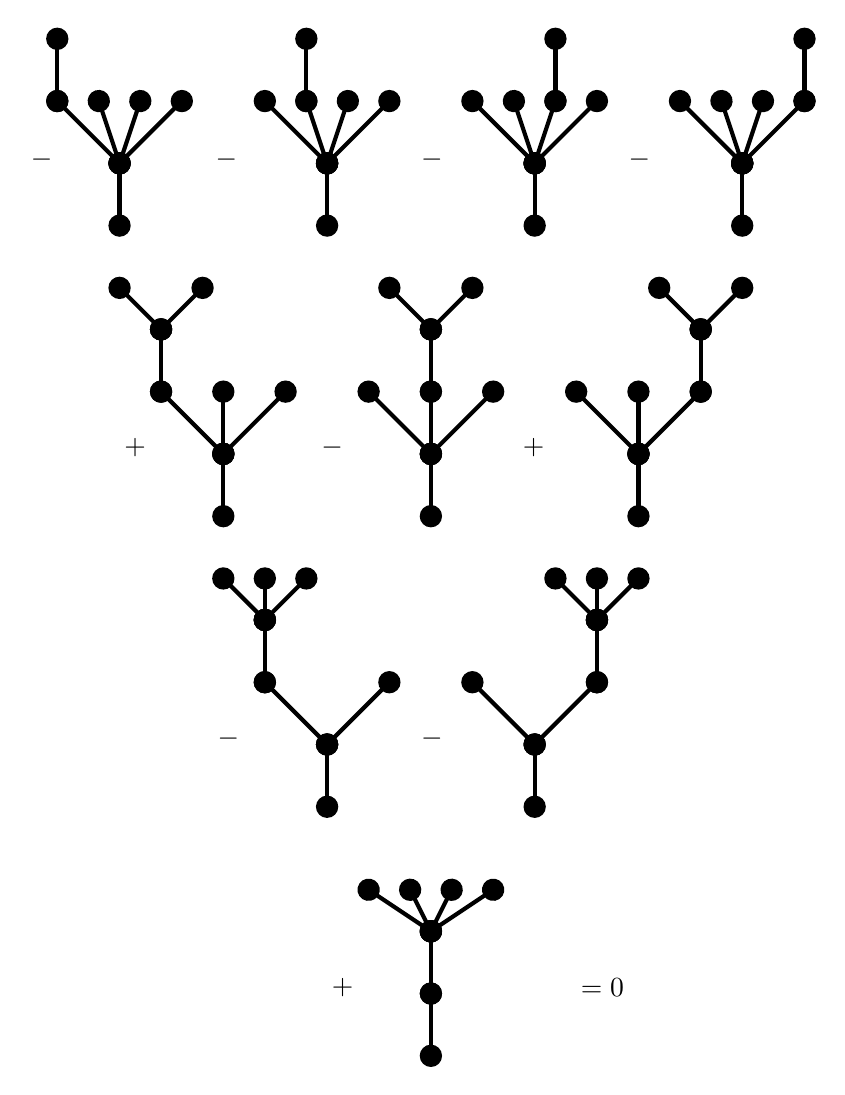
\begin{tikzpicture}[x=0.75pt,y=0.75pt,yscale=-1,xscale=1]
%uncomment if require: \path (0,513); %set diagram left start at 0, and has height of 513

%Straight Lines [id:da7271236022900844] 
\draw [line width=1.5]    (50,70) -- (20,40) ;
\draw [shift={(20,40)}, rotate = 225] [color={rgb, 255:red, 0; green, 0; blue, 0 }  ][fill={rgb, 255:red, 0; green, 0; blue, 0 }  ][line width=1.5]      (0, 0) circle [x radius= 4.36, y radius= 4.36]   ;
\draw [shift={(50,70)}, rotate = 225] [color={rgb, 255:red, 0; green, 0; blue, 0 }  ][fill={rgb, 255:red, 0; green, 0; blue, 0 }  ][line width=1.5]      (0, 0) circle [x radius= 4.36, y radius= 4.36]   ;
%Straight Lines [id:da8829298962249057] 
\draw [line width=1.5]    (50,70) -- (40,40) ;
\draw [shift={(40,40)}, rotate = 251.57] [color={rgb, 255:red, 0; green, 0; blue, 0 }  ][fill={rgb, 255:red, 0; green, 0; blue, 0 }  ][line width=1.5]      (0, 0) circle [x radius= 4.36, y radius= 4.36]   ;
\draw [shift={(50,70)}, rotate = 251.57] [color={rgb, 255:red, 0; green, 0; blue, 0 }  ][fill={rgb, 255:red, 0; green, 0; blue, 0 }  ][line width=1.5]      (0, 0) circle [x radius= 4.36, y radius= 4.36]   ;
%Straight Lines [id:da14019661944022443] 
\draw [line width=1.5]    (50,70) -- (80,40) ;
\draw [shift={(80,40)}, rotate = 315] [color={rgb, 255:red, 0; green, 0; blue, 0 }  ][fill={rgb, 255:red, 0; green, 0; blue, 0 }  ][line width=1.5]      (0, 0) circle [x radius= 4.36, y radius= 4.36]   ;
\draw [shift={(50,70)}, rotate = 315] [color={rgb, 255:red, 0; green, 0; blue, 0 }  ][fill={rgb, 255:red, 0; green, 0; blue, 0 }  ][line width=1.5]      (0, 0) circle [x radius= 4.36, y radius= 4.36]   ;
%Straight Lines [id:da3561053996918748] 
\draw [line width=1.5]    (50,100) -- (50,70) ;
\draw [shift={(50,70)}, rotate = 270] [color={rgb, 255:red, 0; green, 0; blue, 0 }  ][fill={rgb, 255:red, 0; green, 0; blue, 0 }  ][line width=1.5]      (0, 0) circle [x radius= 4.36, y radius= 4.36]   ;
\draw [shift={(50,100)}, rotate = 270] [color={rgb, 255:red, 0; green, 0; blue, 0 }  ][fill={rgb, 255:red, 0; green, 0; blue, 0 }  ][line width=1.5]      (0, 0) circle [x radius= 4.36, y radius= 4.36]   ;
%Straight Lines [id:da12959305658190345] 
\draw [line width=1.5]    (60,40) -- (50,70) ;
\draw [shift={(50,70)}, rotate = 108.43] [color={rgb, 255:red, 0; green, 0; blue, 0 }  ][fill={rgb, 255:red, 0; green, 0; blue, 0 }  ][line width=1.5]      (0, 0) circle [x radius= 4.36, y radius= 4.36]   ;
\draw [shift={(60,40)}, rotate = 108.43] [color={rgb, 255:red, 0; green, 0; blue, 0 }  ][fill={rgb, 255:red, 0; green, 0; blue, 0 }  ][line width=1.5]      (0, 0) circle [x radius= 4.36, y radius= 4.36]   ;
%Straight Lines [id:da17788889705056876] 
\draw [line width=1.5]    (150,70) -- (120,40) ;
\draw [shift={(120,40)}, rotate = 225] [color={rgb, 255:red, 0; green, 0; blue, 0 }  ][fill={rgb, 255:red, 0; green, 0; blue, 0 }  ][line width=1.5]      (0, 0) circle [x radius= 4.36, y radius= 4.36]   ;
\draw [shift={(150,70)}, rotate = 225] [color={rgb, 255:red, 0; green, 0; blue, 0 }  ][fill={rgb, 255:red, 0; green, 0; blue, 0 }  ][line width=1.5]      (0, 0) circle [x radius= 4.36, y radius= 4.36]   ;
%Straight Lines [id:da32726690992182617] 
\draw [line width=1.5]    (150,70) -- (140,40) ;
\draw [shift={(140,40)}, rotate = 251.57] [color={rgb, 255:red, 0; green, 0; blue, 0 }  ][fill={rgb, 255:red, 0; green, 0; blue, 0 }  ][line width=1.5]      (0, 0) circle [x radius= 4.36, y radius= 4.36]   ;
\draw [shift={(150,70)}, rotate = 251.57] [color={rgb, 255:red, 0; green, 0; blue, 0 }  ][fill={rgb, 255:red, 0; green, 0; blue, 0 }  ][line width=1.5]      (0, 0) circle [x radius= 4.36, y radius= 4.36]   ;
%Straight Lines [id:da6529521762459134] 
\draw [line width=1.5]    (150,70) -- (180,40) ;
\draw [shift={(180,40)}, rotate = 315] [color={rgb, 255:red, 0; green, 0; blue, 0 }  ][fill={rgb, 255:red, 0; green, 0; blue, 0 }  ][line width=1.5]      (0, 0) circle [x radius= 4.36, y radius= 4.36]   ;
\draw [shift={(150,70)}, rotate = 315] [color={rgb, 255:red, 0; green, 0; blue, 0 }  ][fill={rgb, 255:red, 0; green, 0; blue, 0 }  ][line width=1.5]      (0, 0) circle [x radius= 4.36, y radius= 4.36]   ;
%Straight Lines [id:da10508941767197344] 
\draw [line width=1.5]    (150,100) -- (150,70) ;
\draw [shift={(150,70)}, rotate = 270] [color={rgb, 255:red, 0; green, 0; blue, 0 }  ][fill={rgb, 255:red, 0; green, 0; blue, 0 }  ][line width=1.5]      (0, 0) circle [x radius= 4.36, y radius= 4.36]   ;
\draw [shift={(150,100)}, rotate = 270] [color={rgb, 255:red, 0; green, 0; blue, 0 }  ][fill={rgb, 255:red, 0; green, 0; blue, 0 }  ][line width=1.5]      (0, 0) circle [x radius= 4.36, y radius= 4.36]   ;
%Straight Lines [id:da6259633442377939] 
\draw [line width=1.5]    (160,40) -- (150,70) ;
\draw [shift={(150,70)}, rotate = 108.43] [color={rgb, 255:red, 0; green, 0; blue, 0 }  ][fill={rgb, 255:red, 0; green, 0; blue, 0 }  ][line width=1.5]      (0, 0) circle [x radius= 4.36, y radius= 4.36]   ;
\draw [shift={(160,40)}, rotate = 108.43] [color={rgb, 255:red, 0; green, 0; blue, 0 }  ][fill={rgb, 255:red, 0; green, 0; blue, 0 }  ][line width=1.5]      (0, 0) circle [x radius= 4.36, y radius= 4.36]   ;
%Straight Lines [id:da18827403823128308] 
\draw [line width=1.5]    (250,70) -- (220,40) ;
\draw [shift={(220,40)}, rotate = 225] [color={rgb, 255:red, 0; green, 0; blue, 0 }  ][fill={rgb, 255:red, 0; green, 0; blue, 0 }  ][line width=1.5]      (0, 0) circle [x radius= 4.36, y radius= 4.36]   ;
\draw [shift={(250,70)}, rotate = 225] [color={rgb, 255:red, 0; green, 0; blue, 0 }  ][fill={rgb, 255:red, 0; green, 0; blue, 0 }  ][line width=1.5]      (0, 0) circle [x radius= 4.36, y radius= 4.36]   ;
%Straight Lines [id:da4416224263321782] 
\draw [line width=1.5]    (250,70) -- (240,40) ;
\draw [shift={(240,40)}, rotate = 251.57] [color={rgb, 255:red, 0; green, 0; blue, 0 }  ][fill={rgb, 255:red, 0; green, 0; blue, 0 }  ][line width=1.5]      (0, 0) circle [x radius= 4.36, y radius= 4.36]   ;
\draw [shift={(250,70)}, rotate = 251.57] [color={rgb, 255:red, 0; green, 0; blue, 0 }  ][fill={rgb, 255:red, 0; green, 0; blue, 0 }  ][line width=1.5]      (0, 0) circle [x radius= 4.36, y radius= 4.36]   ;
%Straight Lines [id:da4912193105487581] 
\draw [line width=1.5]    (250,70) -- (280,40) ;
\draw [shift={(280,40)}, rotate = 315] [color={rgb, 255:red, 0; green, 0; blue, 0 }  ][fill={rgb, 255:red, 0; green, 0; blue, 0 }  ][line width=1.5]      (0, 0) circle [x radius= 4.36, y radius= 4.36]   ;
\draw [shift={(250,70)}, rotate = 315] [color={rgb, 255:red, 0; green, 0; blue, 0 }  ][fill={rgb, 255:red, 0; green, 0; blue, 0 }  ][line width=1.5]      (0, 0) circle [x radius= 4.36, y radius= 4.36]   ;
%Straight Lines [id:da057140828311111225] 
\draw [line width=1.5]    (250,100) -- (250,70) ;
\draw [shift={(250,70)}, rotate = 270] [color={rgb, 255:red, 0; green, 0; blue, 0 }  ][fill={rgb, 255:red, 0; green, 0; blue, 0 }  ][line width=1.5]      (0, 0) circle [x radius= 4.36, y radius= 4.36]   ;
\draw [shift={(250,100)}, rotate = 270] [color={rgb, 255:red, 0; green, 0; blue, 0 }  ][fill={rgb, 255:red, 0; green, 0; blue, 0 }  ][line width=1.5]      (0, 0) circle [x radius= 4.36, y radius= 4.36]   ;
%Straight Lines [id:da6532175337656438] 
\draw [line width=1.5]    (260,40) -- (250,70) ;
\draw [shift={(250,70)}, rotate = 108.43] [color={rgb, 255:red, 0; green, 0; blue, 0 }  ][fill={rgb, 255:red, 0; green, 0; blue, 0 }  ][line width=1.5]      (0, 0) circle [x radius= 4.36, y radius= 4.36]   ;
\draw [shift={(260,40)}, rotate = 108.43] [color={rgb, 255:red, 0; green, 0; blue, 0 }  ][fill={rgb, 255:red, 0; green, 0; blue, 0 }  ][line width=1.5]      (0, 0) circle [x radius= 4.36, y radius= 4.36]   ;
%Straight Lines [id:da9439423309856876] 
\draw [line width=1.5]    (350,70) -- (320,40) ;
\draw [shift={(320,40)}, rotate = 225] [color={rgb, 255:red, 0; green, 0; blue, 0 }  ][fill={rgb, 255:red, 0; green, 0; blue, 0 }  ][line width=1.5]      (0, 0) circle [x radius= 4.36, y radius= 4.36]   ;
\draw [shift={(350,70)}, rotate = 225] [color={rgb, 255:red, 0; green, 0; blue, 0 }  ][fill={rgb, 255:red, 0; green, 0; blue, 0 }  ][line width=1.5]      (0, 0) circle [x radius= 4.36, y radius= 4.36]   ;
%Straight Lines [id:da6793777254659024] 
\draw [line width=1.5]    (350,70) -- (340,40) ;
\draw [shift={(340,40)}, rotate = 251.57] [color={rgb, 255:red, 0; green, 0; blue, 0 }  ][fill={rgb, 255:red, 0; green, 0; blue, 0 }  ][line width=1.5]      (0, 0) circle [x radius= 4.36, y radius= 4.36]   ;
\draw [shift={(350,70)}, rotate = 251.57] [color={rgb, 255:red, 0; green, 0; blue, 0 }  ][fill={rgb, 255:red, 0; green, 0; blue, 0 }  ][line width=1.5]      (0, 0) circle [x radius= 4.36, y radius= 4.36]   ;
%Straight Lines [id:da4673813785992058] 
\draw [line width=1.5]    (350,70) -- (380,40) ;
\draw [shift={(380,40)}, rotate = 315] [color={rgb, 255:red, 0; green, 0; blue, 0 }  ][fill={rgb, 255:red, 0; green, 0; blue, 0 }  ][line width=1.5]      (0, 0) circle [x radius= 4.36, y radius= 4.36]   ;
\draw [shift={(350,70)}, rotate = 315] [color={rgb, 255:red, 0; green, 0; blue, 0 }  ][fill={rgb, 255:red, 0; green, 0; blue, 0 }  ][line width=1.5]      (0, 0) circle [x radius= 4.36, y radius= 4.36]   ;
%Straight Lines [id:da2972746595471605] 
\draw [line width=1.5]    (350,100) -- (350,70) ;
\draw [shift={(350,70)}, rotate = 270] [color={rgb, 255:red, 0; green, 0; blue, 0 }  ][fill={rgb, 255:red, 0; green, 0; blue, 0 }  ][line width=1.5]      (0, 0) circle [x radius= 4.36, y radius= 4.36]   ;
\draw [shift={(350,100)}, rotate = 270] [color={rgb, 255:red, 0; green, 0; blue, 0 }  ][fill={rgb, 255:red, 0; green, 0; blue, 0 }  ][line width=1.5]      (0, 0) circle [x radius= 4.36, y radius= 4.36]   ;
%Straight Lines [id:da526738135792] 
\draw [line width=1.5]    (360,40) -- (350,70) ;
\draw [shift={(350,70)}, rotate = 108.43] [color={rgb, 255:red, 0; green, 0; blue, 0 }  ][fill={rgb, 255:red, 0; green, 0; blue, 0 }  ][line width=1.5]      (0, 0) circle [x radius= 4.36, y radius= 4.36]   ;
\draw [shift={(360,40)}, rotate = 108.43] [color={rgb, 255:red, 0; green, 0; blue, 0 }  ][fill={rgb, 255:red, 0; green, 0; blue, 0 }  ][line width=1.5]      (0, 0) circle [x radius= 4.36, y radius= 4.36]   ;
%Straight Lines [id:da3439286430792807] 
\draw [line width=1.5]    (20,40) -- (20,10) ;
\draw [shift={(20,10)}, rotate = 270] [color={rgb, 255:red, 0; green, 0; blue, 0 }  ][fill={rgb, 255:red, 0; green, 0; blue, 0 }  ][line width=1.5]      (0, 0) circle [x radius= 4.36, y radius= 4.36]   ;
\draw [shift={(20,40)}, rotate = 270] [color={rgb, 255:red, 0; green, 0; blue, 0 }  ][fill={rgb, 255:red, 0; green, 0; blue, 0 }  ][line width=1.5]      (0, 0) circle [x radius= 4.36, y radius= 4.36]   ;
%Straight Lines [id:da027749002350105467] 
\draw [line width=1.5]    (140,40) -- (140,10) ;
\draw [shift={(140,10)}, rotate = 270] [color={rgb, 255:red, 0; green, 0; blue, 0 }  ][fill={rgb, 255:red, 0; green, 0; blue, 0 }  ][line width=1.5]      (0, 0) circle [x radius= 4.36, y radius= 4.36]   ;
\draw [shift={(140,40)}, rotate = 270] [color={rgb, 255:red, 0; green, 0; blue, 0 }  ][fill={rgb, 255:red, 0; green, 0; blue, 0 }  ][line width=1.5]      (0, 0) circle [x radius= 4.36, y radius= 4.36]   ;
%Straight Lines [id:da4141601555763963] 
\draw [line width=1.5]    (260,40) -- (260,10) ;
\draw [shift={(260,10)}, rotate = 270] [color={rgb, 255:red, 0; green, 0; blue, 0 }  ][fill={rgb, 255:red, 0; green, 0; blue, 0 }  ][line width=1.5]      (0, 0) circle [x radius= 4.36, y radius= 4.36]   ;
\draw [shift={(260,40)}, rotate = 270] [color={rgb, 255:red, 0; green, 0; blue, 0 }  ][fill={rgb, 255:red, 0; green, 0; blue, 0 }  ][line width=1.5]      (0, 0) circle [x radius= 4.36, y radius= 4.36]   ;
%Straight Lines [id:da8143971343614638] 
\draw [line width=1.5]    (380,40) -- (380,10) ;
\draw [shift={(380,10)}, rotate = 270] [color={rgb, 255:red, 0; green, 0; blue, 0 }  ][fill={rgb, 255:red, 0; green, 0; blue, 0 }  ][line width=1.5]      (0, 0) circle [x radius= 4.36, y radius= 4.36]   ;
\draw [shift={(380,40)}, rotate = 270] [color={rgb, 255:red, 0; green, 0; blue, 0 }  ][fill={rgb, 255:red, 0; green, 0; blue, 0 }  ][line width=1.5]      (0, 0) circle [x radius= 4.36, y radius= 4.36]   ;
%Straight Lines [id:da5027840919946027] 
\draw [line width=1.5]    (100,210) -- (70,180) ;
\draw [shift={(70,180)}, rotate = 225] [color={rgb, 255:red, 0; green, 0; blue, 0 }  ][fill={rgb, 255:red, 0; green, 0; blue, 0 }  ][line width=1.5]      (0, 0) circle [x radius= 4.36, y radius= 4.36]   ;
\draw [shift={(100,210)}, rotate = 225] [color={rgb, 255:red, 0; green, 0; blue, 0 }  ][fill={rgb, 255:red, 0; green, 0; blue, 0 }  ][line width=1.5]      (0, 0) circle [x radius= 4.36, y radius= 4.36]   ;
%Straight Lines [id:da012169408330350517] 
\draw [line width=1.5]    (100,210) -- (100,180) ;
\draw [shift={(100,180)}, rotate = 270] [color={rgb, 255:red, 0; green, 0; blue, 0 }  ][fill={rgb, 255:red, 0; green, 0; blue, 0 }  ][line width=1.5]      (0, 0) circle [x radius= 4.36, y radius= 4.36]   ;
\draw [shift={(100,210)}, rotate = 270] [color={rgb, 255:red, 0; green, 0; blue, 0 }  ][fill={rgb, 255:red, 0; green, 0; blue, 0 }  ][line width=1.5]      (0, 0) circle [x radius= 4.36, y radius= 4.36]   ;
%Straight Lines [id:da3794956070144304] 
\draw [line width=1.5]    (100,210) -- (130,180) ;
\draw [shift={(130,180)}, rotate = 315] [color={rgb, 255:red, 0; green, 0; blue, 0 }  ][fill={rgb, 255:red, 0; green, 0; blue, 0 }  ][line width=1.5]      (0, 0) circle [x radius= 4.36, y radius= 4.36]   ;
\draw [shift={(100,210)}, rotate = 315] [color={rgb, 255:red, 0; green, 0; blue, 0 }  ][fill={rgb, 255:red, 0; green, 0; blue, 0 }  ][line width=1.5]      (0, 0) circle [x radius= 4.36, y radius= 4.36]   ;
%Straight Lines [id:da8996197602070666] 
\draw [line width=1.5]    (100,240) -- (100,210) ;
\draw [shift={(100,210)}, rotate = 270] [color={rgb, 255:red, 0; green, 0; blue, 0 }  ][fill={rgb, 255:red, 0; green, 0; blue, 0 }  ][line width=1.5]      (0, 0) circle [x radius= 4.36, y radius= 4.36]   ;
\draw [shift={(100,240)}, rotate = 270] [color={rgb, 255:red, 0; green, 0; blue, 0 }  ][fill={rgb, 255:red, 0; green, 0; blue, 0 }  ][line width=1.5]      (0, 0) circle [x radius= 4.36, y radius= 4.36]   ;
%Straight Lines [id:da1531842966441921] 
\draw [line width=1.5]    (70,150) -- (50,130) ;
\draw [shift={(50,130)}, rotate = 225] [color={rgb, 255:red, 0; green, 0; blue, 0 }  ][fill={rgb, 255:red, 0; green, 0; blue, 0 }  ][line width=1.5]      (0, 0) circle [x radius= 4.36, y radius= 4.36]   ;
\draw [shift={(70,150)}, rotate = 225] [color={rgb, 255:red, 0; green, 0; blue, 0 }  ][fill={rgb, 255:red, 0; green, 0; blue, 0 }  ][line width=1.5]      (0, 0) circle [x radius= 4.36, y radius= 4.36]   ;
%Straight Lines [id:da5635603151723407] 
\draw [line width=1.5]    (70,150) -- (90,130) ;
\draw [shift={(90,130)}, rotate = 315] [color={rgb, 255:red, 0; green, 0; blue, 0 }  ][fill={rgb, 255:red, 0; green, 0; blue, 0 }  ][line width=1.5]      (0, 0) circle [x radius= 4.36, y radius= 4.36]   ;
\draw [shift={(70,150)}, rotate = 315] [color={rgb, 255:red, 0; green, 0; blue, 0 }  ][fill={rgb, 255:red, 0; green, 0; blue, 0 }  ][line width=1.5]      (0, 0) circle [x radius= 4.36, y radius= 4.36]   ;
%Straight Lines [id:da37599967010410107] 
\draw [line width=1.5]    (70,180) -- (70,150) ;
\draw [shift={(70,150)}, rotate = 270] [color={rgb, 255:red, 0; green, 0; blue, 0 }  ][fill={rgb, 255:red, 0; green, 0; blue, 0 }  ][line width=1.5]      (0, 0) circle [x radius= 4.36, y radius= 4.36]   ;
\draw [shift={(70,180)}, rotate = 270] [color={rgb, 255:red, 0; green, 0; blue, 0 }  ][fill={rgb, 255:red, 0; green, 0; blue, 0 }  ][line width=1.5]      (0, 0) circle [x radius= 4.36, y radius= 4.36]   ;
%Straight Lines [id:da698265177656928] 
\draw [line width=1.5]    (200,210) -- (170,180) ;
\draw [shift={(170,180)}, rotate = 225] [color={rgb, 255:red, 0; green, 0; blue, 0 }  ][fill={rgb, 255:red, 0; green, 0; blue, 0 }  ][line width=1.5]      (0, 0) circle [x radius= 4.36, y radius= 4.36]   ;
\draw [shift={(200,210)}, rotate = 225] [color={rgb, 255:red, 0; green, 0; blue, 0 }  ][fill={rgb, 255:red, 0; green, 0; blue, 0 }  ][line width=1.5]      (0, 0) circle [x radius= 4.36, y radius= 4.36]   ;
%Straight Lines [id:da049456703112388256] 
\draw [line width=1.5]    (200,210) -- (200,180) ;
\draw [shift={(200,180)}, rotate = 270] [color={rgb, 255:red, 0; green, 0; blue, 0 }  ][fill={rgb, 255:red, 0; green, 0; blue, 0 }  ][line width=1.5]      (0, 0) circle [x radius= 4.36, y radius= 4.36]   ;
\draw [shift={(200,210)}, rotate = 270] [color={rgb, 255:red, 0; green, 0; blue, 0 }  ][fill={rgb, 255:red, 0; green, 0; blue, 0 }  ][line width=1.5]      (0, 0) circle [x radius= 4.36, y radius= 4.36]   ;
%Straight Lines [id:da19781405329398405] 
\draw [line width=1.5]    (200,210) -- (230,180) ;
\draw [shift={(230,180)}, rotate = 315] [color={rgb, 255:red, 0; green, 0; blue, 0 }  ][fill={rgb, 255:red, 0; green, 0; blue, 0 }  ][line width=1.5]      (0, 0) circle [x radius= 4.36, y radius= 4.36]   ;
\draw [shift={(200,210)}, rotate = 315] [color={rgb, 255:red, 0; green, 0; blue, 0 }  ][fill={rgb, 255:red, 0; green, 0; blue, 0 }  ][line width=1.5]      (0, 0) circle [x radius= 4.36, y radius= 4.36]   ;
%Straight Lines [id:da9771660287757578] 
\draw [line width=1.5]    (200,240) -- (200,210) ;
\draw [shift={(200,210)}, rotate = 270] [color={rgb, 255:red, 0; green, 0; blue, 0 }  ][fill={rgb, 255:red, 0; green, 0; blue, 0 }  ][line width=1.5]      (0, 0) circle [x radius= 4.36, y radius= 4.36]   ;
\draw [shift={(200,240)}, rotate = 270] [color={rgb, 255:red, 0; green, 0; blue, 0 }  ][fill={rgb, 255:red, 0; green, 0; blue, 0 }  ][line width=1.5]      (0, 0) circle [x radius= 4.36, y radius= 4.36]   ;
%Straight Lines [id:da8050669462477833] 
\draw [line width=1.5]    (200,150) -- (180,130) ;
\draw [shift={(180,130)}, rotate = 225] [color={rgb, 255:red, 0; green, 0; blue, 0 }  ][fill={rgb, 255:red, 0; green, 0; blue, 0 }  ][line width=1.5]      (0, 0) circle [x radius= 4.36, y radius= 4.36]   ;
\draw [shift={(200,150)}, rotate = 225] [color={rgb, 255:red, 0; green, 0; blue, 0 }  ][fill={rgb, 255:red, 0; green, 0; blue, 0 }  ][line width=1.5]      (0, 0) circle [x radius= 4.36, y radius= 4.36]   ;
%Straight Lines [id:da4433467710630703] 
\draw [line width=1.5]    (200,150) -- (220,130) ;
\draw [shift={(220,130)}, rotate = 315] [color={rgb, 255:red, 0; green, 0; blue, 0 }  ][fill={rgb, 255:red, 0; green, 0; blue, 0 }  ][line width=1.5]      (0, 0) circle [x radius= 4.36, y radius= 4.36]   ;
\draw [shift={(200,150)}, rotate = 315] [color={rgb, 255:red, 0; green, 0; blue, 0 }  ][fill={rgb, 255:red, 0; green, 0; blue, 0 }  ][line width=1.5]      (0, 0) circle [x radius= 4.36, y radius= 4.36]   ;
%Straight Lines [id:da01581391478939298] 
\draw [line width=1.5]    (200,180) -- (200,150) ;
\draw [shift={(200,150)}, rotate = 270] [color={rgb, 255:red, 0; green, 0; blue, 0 }  ][fill={rgb, 255:red, 0; green, 0; blue, 0 }  ][line width=1.5]      (0, 0) circle [x radius= 4.36, y radius= 4.36]   ;
\draw [shift={(200,180)}, rotate = 270] [color={rgb, 255:red, 0; green, 0; blue, 0 }  ][fill={rgb, 255:red, 0; green, 0; blue, 0 }  ][line width=1.5]      (0, 0) circle [x radius= 4.36, y radius= 4.36]   ;
%Straight Lines [id:da39290163971213876] 
\draw [line width=1.5]    (300,210) -- (270,180) ;
\draw [shift={(270,180)}, rotate = 225] [color={rgb, 255:red, 0; green, 0; blue, 0 }  ][fill={rgb, 255:red, 0; green, 0; blue, 0 }  ][line width=1.5]      (0, 0) circle [x radius= 4.36, y radius= 4.36]   ;
\draw [shift={(300,210)}, rotate = 225] [color={rgb, 255:red, 0; green, 0; blue, 0 }  ][fill={rgb, 255:red, 0; green, 0; blue, 0 }  ][line width=1.5]      (0, 0) circle [x radius= 4.36, y radius= 4.36]   ;
%Straight Lines [id:da6585976068778385] 
\draw [line width=1.5]    (300,210) -- (300,180) ;
\draw [shift={(300,180)}, rotate = 270] [color={rgb, 255:red, 0; green, 0; blue, 0 }  ][fill={rgb, 255:red, 0; green, 0; blue, 0 }  ][line width=1.5]      (0, 0) circle [x radius= 4.36, y radius= 4.36]   ;
\draw [shift={(300,210)}, rotate = 270] [color={rgb, 255:red, 0; green, 0; blue, 0 }  ][fill={rgb, 255:red, 0; green, 0; blue, 0 }  ][line width=1.5]      (0, 0) circle [x radius= 4.36, y radius= 4.36]   ;
%Straight Lines [id:da08497570166304391] 
\draw [line width=1.5]    (300,210) -- (330,180) ;
\draw [shift={(330,180)}, rotate = 315] [color={rgb, 255:red, 0; green, 0; blue, 0 }  ][fill={rgb, 255:red, 0; green, 0; blue, 0 }  ][line width=1.5]      (0, 0) circle [x radius= 4.36, y radius= 4.36]   ;
\draw [shift={(300,210)}, rotate = 315] [color={rgb, 255:red, 0; green, 0; blue, 0 }  ][fill={rgb, 255:red, 0; green, 0; blue, 0 }  ][line width=1.5]      (0, 0) circle [x radius= 4.36, y radius= 4.36]   ;
%Straight Lines [id:da6049966997095673] 
\draw [line width=1.5]    (300,240) -- (300,210) ;
\draw [shift={(300,210)}, rotate = 270] [color={rgb, 255:red, 0; green, 0; blue, 0 }  ][fill={rgb, 255:red, 0; green, 0; blue, 0 }  ][line width=1.5]      (0, 0) circle [x radius= 4.36, y radius= 4.36]   ;
\draw [shift={(300,240)}, rotate = 270] [color={rgb, 255:red, 0; green, 0; blue, 0 }  ][fill={rgb, 255:red, 0; green, 0; blue, 0 }  ][line width=1.5]      (0, 0) circle [x radius= 4.36, y radius= 4.36]   ;
%Straight Lines [id:da3027007292774597] 
\draw [line width=1.5]    (330,150) -- (310,130) ;
\draw [shift={(310,130)}, rotate = 225] [color={rgb, 255:red, 0; green, 0; blue, 0 }  ][fill={rgb, 255:red, 0; green, 0; blue, 0 }  ][line width=1.5]      (0, 0) circle [x radius= 4.36, y radius= 4.36]   ;
\draw [shift={(330,150)}, rotate = 225] [color={rgb, 255:red, 0; green, 0; blue, 0 }  ][fill={rgb, 255:red, 0; green, 0; blue, 0 }  ][line width=1.5]      (0, 0) circle [x radius= 4.36, y radius= 4.36]   ;
%Straight Lines [id:da8425409794662362] 
\draw [line width=1.5]    (330,150) -- (350,130) ;
\draw [shift={(350,130)}, rotate = 315] [color={rgb, 255:red, 0; green, 0; blue, 0 }  ][fill={rgb, 255:red, 0; green, 0; blue, 0 }  ][line width=1.5]      (0, 0) circle [x radius= 4.36, y radius= 4.36]   ;
\draw [shift={(330,150)}, rotate = 315] [color={rgb, 255:red, 0; green, 0; blue, 0 }  ][fill={rgb, 255:red, 0; green, 0; blue, 0 }  ][line width=1.5]      (0, 0) circle [x radius= 4.36, y radius= 4.36]   ;
%Straight Lines [id:da6597509617717114] 
\draw [line width=1.5]    (330,180) -- (330,150) ;
\draw [shift={(330,150)}, rotate = 270] [color={rgb, 255:red, 0; green, 0; blue, 0 }  ][fill={rgb, 255:red, 0; green, 0; blue, 0 }  ][line width=1.5]      (0, 0) circle [x radius= 4.36, y radius= 4.36]   ;
\draw [shift={(330,180)}, rotate = 270] [color={rgb, 255:red, 0; green, 0; blue, 0 }  ][fill={rgb, 255:red, 0; green, 0; blue, 0 }  ][line width=1.5]      (0, 0) circle [x radius= 4.36, y radius= 4.36]   ;
%Straight Lines [id:da4925140669754495] 
\draw [line width=1.5]    (150,350) -- (120,320) ;
\draw [shift={(120,320)}, rotate = 225] [color={rgb, 255:red, 0; green, 0; blue, 0 }  ][fill={rgb, 255:red, 0; green, 0; blue, 0 }  ][line width=1.5]      (0, 0) circle [x radius= 4.36, y radius= 4.36]   ;
\draw [shift={(150,350)}, rotate = 225] [color={rgb, 255:red, 0; green, 0; blue, 0 }  ][fill={rgb, 255:red, 0; green, 0; blue, 0 }  ][line width=1.5]      (0, 0) circle [x radius= 4.36, y radius= 4.36]   ;
%Straight Lines [id:da22967712249663763] 
\draw [line width=1.5]    (150,350) -- (180,320) ;
\draw [shift={(180,320)}, rotate = 315] [color={rgb, 255:red, 0; green, 0; blue, 0 }  ][fill={rgb, 255:red, 0; green, 0; blue, 0 }  ][line width=1.5]      (0, 0) circle [x radius= 4.36, y radius= 4.36]   ;
\draw [shift={(150,350)}, rotate = 315] [color={rgb, 255:red, 0; green, 0; blue, 0 }  ][fill={rgb, 255:red, 0; green, 0; blue, 0 }  ][line width=1.5]      (0, 0) circle [x radius= 4.36, y radius= 4.36]   ;
%Straight Lines [id:da18647592300425853] 
\draw [line width=1.5]    (150,380) -- (150,350) ;
\draw [shift={(150,350)}, rotate = 270] [color={rgb, 255:red, 0; green, 0; blue, 0 }  ][fill={rgb, 255:red, 0; green, 0; blue, 0 }  ][line width=1.5]      (0, 0) circle [x radius= 4.36, y radius= 4.36]   ;
\draw [shift={(150,380)}, rotate = 270] [color={rgb, 255:red, 0; green, 0; blue, 0 }  ][fill={rgb, 255:red, 0; green, 0; blue, 0 }  ][line width=1.5]      (0, 0) circle [x radius= 4.36, y radius= 4.36]   ;
%Straight Lines [id:da046931680579429536] 
\draw [line width=1.5]    (250,350) -- (220,320) ;
\draw [shift={(220,320)}, rotate = 225] [color={rgb, 255:red, 0; green, 0; blue, 0 }  ][fill={rgb, 255:red, 0; green, 0; blue, 0 }  ][line width=1.5]      (0, 0) circle [x radius= 4.36, y radius= 4.36]   ;
\draw [shift={(250,350)}, rotate = 225] [color={rgb, 255:red, 0; green, 0; blue, 0 }  ][fill={rgb, 255:red, 0; green, 0; blue, 0 }  ][line width=1.5]      (0, 0) circle [x radius= 4.36, y radius= 4.36]   ;
%Straight Lines [id:da2728002796290594] 
\draw [line width=1.5]    (250,350) -- (280,320) ;
\draw [shift={(280,320)}, rotate = 315] [color={rgb, 255:red, 0; green, 0; blue, 0 }  ][fill={rgb, 255:red, 0; green, 0; blue, 0 }  ][line width=1.5]      (0, 0) circle [x radius= 4.36, y radius= 4.36]   ;
\draw [shift={(250,350)}, rotate = 315] [color={rgb, 255:red, 0; green, 0; blue, 0 }  ][fill={rgb, 255:red, 0; green, 0; blue, 0 }  ][line width=1.5]      (0, 0) circle [x radius= 4.36, y radius= 4.36]   ;
%Straight Lines [id:da48284795242627854] 
\draw [line width=1.5]    (250,380) -- (250,350) ;
\draw [shift={(250,350)}, rotate = 270] [color={rgb, 255:red, 0; green, 0; blue, 0 }  ][fill={rgb, 255:red, 0; green, 0; blue, 0 }  ][line width=1.5]      (0, 0) circle [x radius= 4.36, y radius= 4.36]   ;
\draw [shift={(250,380)}, rotate = 270] [color={rgb, 255:red, 0; green, 0; blue, 0 }  ][fill={rgb, 255:red, 0; green, 0; blue, 0 }  ][line width=1.5]      (0, 0) circle [x radius= 4.36, y radius= 4.36]   ;
%Straight Lines [id:da3493008605600656] 
\draw [line width=1.5]    (120,290) -- (100,270) ;
\draw [shift={(100,270)}, rotate = 225] [color={rgb, 255:red, 0; green, 0; blue, 0 }  ][fill={rgb, 255:red, 0; green, 0; blue, 0 }  ][line width=1.5]      (0, 0) circle [x radius= 4.36, y radius= 4.36]   ;
\draw [shift={(120,290)}, rotate = 225] [color={rgb, 255:red, 0; green, 0; blue, 0 }  ][fill={rgb, 255:red, 0; green, 0; blue, 0 }  ][line width=1.5]      (0, 0) circle [x radius= 4.36, y radius= 4.36]   ;
%Straight Lines [id:da7800084523238568] 
\draw [line width=1.5]    (120,290) -- (120,270) ;
\draw [shift={(120,270)}, rotate = 270] [color={rgb, 255:red, 0; green, 0; blue, 0 }  ][fill={rgb, 255:red, 0; green, 0; blue, 0 }  ][line width=1.5]      (0, 0) circle [x radius= 4.36, y radius= 4.36]   ;
\draw [shift={(120,290)}, rotate = 270] [color={rgb, 255:red, 0; green, 0; blue, 0 }  ][fill={rgb, 255:red, 0; green, 0; blue, 0 }  ][line width=1.5]      (0, 0) circle [x radius= 4.36, y radius= 4.36]   ;
%Straight Lines [id:da1533956199450981] 
\draw [line width=1.5]    (120,290) -- (140,270) ;
\draw [shift={(140,270)}, rotate = 315] [color={rgb, 255:red, 0; green, 0; blue, 0 }  ][fill={rgb, 255:red, 0; green, 0; blue, 0 }  ][line width=1.5]      (0, 0) circle [x radius= 4.36, y radius= 4.36]   ;
\draw [shift={(120,290)}, rotate = 315] [color={rgb, 255:red, 0; green, 0; blue, 0 }  ][fill={rgb, 255:red, 0; green, 0; blue, 0 }  ][line width=1.5]      (0, 0) circle [x radius= 4.36, y radius= 4.36]   ;
%Straight Lines [id:da6924842976379457] 
\draw [line width=1.5]    (120,320) -- (120,290) ;
\draw [shift={(120,290)}, rotate = 270] [color={rgb, 255:red, 0; green, 0; blue, 0 }  ][fill={rgb, 255:red, 0; green, 0; blue, 0 }  ][line width=1.5]      (0, 0) circle [x radius= 4.36, y radius= 4.36]   ;
\draw [shift={(120,320)}, rotate = 270] [color={rgb, 255:red, 0; green, 0; blue, 0 }  ][fill={rgb, 255:red, 0; green, 0; blue, 0 }  ][line width=1.5]      (0, 0) circle [x radius= 4.36, y radius= 4.36]   ;
%Straight Lines [id:da7782455529560655] 
\draw [line width=1.5]    (280,290) -- (260,270) ;
\draw [shift={(260,270)}, rotate = 225] [color={rgb, 255:red, 0; green, 0; blue, 0 }  ][fill={rgb, 255:red, 0; green, 0; blue, 0 }  ][line width=1.5]      (0, 0) circle [x radius= 4.36, y radius= 4.36]   ;
\draw [shift={(280,290)}, rotate = 225] [color={rgb, 255:red, 0; green, 0; blue, 0 }  ][fill={rgb, 255:red, 0; green, 0; blue, 0 }  ][line width=1.5]      (0, 0) circle [x radius= 4.36, y radius= 4.36]   ;
%Straight Lines [id:da25917615306254826] 
\draw [line width=1.5]    (280,290) -- (280,270) ;
\draw [shift={(280,270)}, rotate = 270] [color={rgb, 255:red, 0; green, 0; blue, 0 }  ][fill={rgb, 255:red, 0; green, 0; blue, 0 }  ][line width=1.5]      (0, 0) circle [x radius= 4.36, y radius= 4.36]   ;
\draw [shift={(280,290)}, rotate = 270] [color={rgb, 255:red, 0; green, 0; blue, 0 }  ][fill={rgb, 255:red, 0; green, 0; blue, 0 }  ][line width=1.5]      (0, 0) circle [x radius= 4.36, y radius= 4.36]   ;
%Straight Lines [id:da0631244877784558] 
\draw [line width=1.5]    (280,290) -- (300,270) ;
\draw [shift={(300,270)}, rotate = 315] [color={rgb, 255:red, 0; green, 0; blue, 0 }  ][fill={rgb, 255:red, 0; green, 0; blue, 0 }  ][line width=1.5]      (0, 0) circle [x radius= 4.36, y radius= 4.36]   ;
\draw [shift={(280,290)}, rotate = 315] [color={rgb, 255:red, 0; green, 0; blue, 0 }  ][fill={rgb, 255:red, 0; green, 0; blue, 0 }  ][line width=1.5]      (0, 0) circle [x radius= 4.36, y radius= 4.36]   ;
%Straight Lines [id:da4893375854965143] 
\draw [line width=1.5]    (280,320) -- (280,290) ;
\draw [shift={(280,290)}, rotate = 270] [color={rgb, 255:red, 0; green, 0; blue, 0 }  ][fill={rgb, 255:red, 0; green, 0; blue, 0 }  ][line width=1.5]      (0, 0) circle [x radius= 4.36, y radius= 4.36]   ;
\draw [shift={(280,320)}, rotate = 270] [color={rgb, 255:red, 0; green, 0; blue, 0 }  ][fill={rgb, 255:red, 0; green, 0; blue, 0 }  ][line width=1.5]      (0, 0) circle [x radius= 4.36, y radius= 4.36]   ;
%Straight Lines [id:da7745941617276062] 
\draw [line width=1.5]    (200,440) -- (170,420) ;
\draw [shift={(170,420)}, rotate = 213.69] [color={rgb, 255:red, 0; green, 0; blue, 0 }  ][fill={rgb, 255:red, 0; green, 0; blue, 0 }  ][line width=1.5]      (0, 0) circle [x radius= 4.36, y radius= 4.36]   ;
\draw [shift={(200,440)}, rotate = 213.69] [color={rgb, 255:red, 0; green, 0; blue, 0 }  ][fill={rgb, 255:red, 0; green, 0; blue, 0 }  ][line width=1.5]      (0, 0) circle [x radius= 4.36, y radius= 4.36]   ;
%Straight Lines [id:da5529629697237282] 
\draw [line width=1.5]    (200,440) -- (190,420) ;
\draw [shift={(190,420)}, rotate = 243.43] [color={rgb, 255:red, 0; green, 0; blue, 0 }  ][fill={rgb, 255:red, 0; green, 0; blue, 0 }  ][line width=1.5]      (0, 0) circle [x radius= 4.36, y radius= 4.36]   ;
\draw [shift={(200,440)}, rotate = 243.43] [color={rgb, 255:red, 0; green, 0; blue, 0 }  ][fill={rgb, 255:red, 0; green, 0; blue, 0 }  ][line width=1.5]      (0, 0) circle [x radius= 4.36, y radius= 4.36]   ;
%Straight Lines [id:da7912065392766896] 
\draw [line width=1.5]    (200,440) -- (230,420) ;
\draw [shift={(230,420)}, rotate = 326.31] [color={rgb, 255:red, 0; green, 0; blue, 0 }  ][fill={rgb, 255:red, 0; green, 0; blue, 0 }  ][line width=1.5]      (0, 0) circle [x radius= 4.36, y radius= 4.36]   ;
\draw [shift={(200,440)}, rotate = 326.31] [color={rgb, 255:red, 0; green, 0; blue, 0 }  ][fill={rgb, 255:red, 0; green, 0; blue, 0 }  ][line width=1.5]      (0, 0) circle [x radius= 4.36, y radius= 4.36]   ;
%Straight Lines [id:da10916285074247245] 
\draw [line width=1.5]    (200,470) -- (200,440) ;
\draw [shift={(200,440)}, rotate = 270] [color={rgb, 255:red, 0; green, 0; blue, 0 }  ][fill={rgb, 255:red, 0; green, 0; blue, 0 }  ][line width=1.5]      (0, 0) circle [x radius= 4.36, y radius= 4.36]   ;
\draw [shift={(200,470)}, rotate = 270] [color={rgb, 255:red, 0; green, 0; blue, 0 }  ][fill={rgb, 255:red, 0; green, 0; blue, 0 }  ][line width=1.5]      (0, 0) circle [x radius= 4.36, y radius= 4.36]   ;
%Straight Lines [id:da15882706355126386] 
\draw [line width=1.5]    (210,420) -- (200,440) ;
\draw [shift={(200,440)}, rotate = 116.57] [color={rgb, 255:red, 0; green, 0; blue, 0 }  ][fill={rgb, 255:red, 0; green, 0; blue, 0 }  ][line width=1.5]      (0, 0) circle [x radius= 4.36, y radius= 4.36]   ;
\draw [shift={(210,420)}, rotate = 116.57] [color={rgb, 255:red, 0; green, 0; blue, 0 }  ][fill={rgb, 255:red, 0; green, 0; blue, 0 }  ][line width=1.5]      (0, 0) circle [x radius= 4.36, y radius= 4.36]   ;
%Straight Lines [id:da9824487516429941] 
\draw [line width=1.5]    (200,500) -- (200,470) ;
\draw [shift={(200,470)}, rotate = 270] [color={rgb, 255:red, 0; green, 0; blue, 0 }  ][fill={rgb, 255:red, 0; green, 0; blue, 0 }  ][line width=1.5]      (0, 0) circle [x radius= 4.36, y radius= 4.36]   ;
\draw [shift={(200,500)}, rotate = 270] [color={rgb, 255:red, 0; green, 0; blue, 0 }  ][fill={rgb, 255:red, 0; green, 0; blue, 0 }  ][line width=1.5]      (0, 0) circle [x radius= 4.36, y radius= 4.36]   ;

% Text Node
\draw (6,62.4) node [anchor=north west][inner sep=0.75pt]    {$-$};
% Text Node
\draw (95,62.4) node [anchor=north west][inner sep=0.75pt]    {$-$};
% Text Node
\draw (194,62.4) node [anchor=north west][inner sep=0.75pt]    {$-$};
% Text Node
\draw (294,62.4) node [anchor=north west][inner sep=0.75pt]    {$-$};
% Text Node
\draw (146,201.4) node [anchor=north west][inner sep=0.75pt]    {$-$};
% Text Node
\draw (51,201.4) node [anchor=north west][inner sep=0.75pt]    {$+$};
% Text Node
\draw (243,201.4) node [anchor=north west][inner sep=0.75pt]    {$+$};
% Text Node
\draw (96,341.4) node [anchor=north west][inner sep=0.75pt]    {$-$};
% Text Node
\draw (194,341.4) node [anchor=north west][inner sep=0.75pt]    {$-$};
% Text Node
\draw (151,461.4) node [anchor=north west][inner sep=0.75pt]    {$+$};
% Text Node
\draw (271,461.4) node [anchor=north west][inner sep=0.75pt]    {$=0$};


\end{tikzpicture}    
\end{center}


\subsubsection{Rooted trees for DG-algebras}

Since we know that a DG-algebra can be though of as an $\A$-algebra where $m_n = 0$ for all $n\geq 3$, we can explicitly write out all the relations we have in a DG-algebra using these trees. The $n=1$ relation is again given by



% The first Stasheff identity for DG algebras using trees

\begin{center}
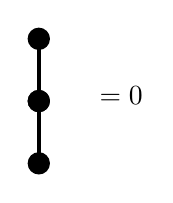
\begin{tikzpicture}[x=0.75pt,y=0.75pt,yscale=-1,xscale=1]
%uncomment if require: \path (0,513); %set diagram left start at 0, and has height of 513

%Straight Lines [id:da5455092391586145] 
\draw [line width=1.5]    (40,60) -- (40,30) ;
\draw [shift={(40,30)}, rotate = 270] [color={rgb, 255:red, 0; green, 0; blue, 0 }  ][fill={rgb, 255:red, 0; green, 0; blue, 0 }  ][line width=1.5]      (0, 0) circle [x radius= 4.36, y radius= 4.36]   ;
\draw [shift={(40,60)}, rotate = 270] [color={rgb, 255:red, 0; green, 0; blue, 0 }  ][fill={rgb, 255:red, 0; green, 0; blue, 0 }  ][line width=1.5]      (0, 0) circle [x radius= 4.36, y radius= 4.36]   ;
%Straight Lines [id:da552453933363283] 
\draw [line width=1.5]    (40,90) -- (40,60) ;
\draw [shift={(40,60)}, rotate = 270] [color={rgb, 255:red, 0; green, 0; blue, 0 }  ][fill={rgb, 255:red, 0; green, 0; blue, 0 }  ][line width=1.5]      (0, 0) circle [x radius= 4.36, y radius= 4.36]   ;
\draw [shift={(40,90)}, rotate = 270] [color={rgb, 255:red, 0; green, 0; blue, 0 }  ][fill={rgb, 255:red, 0; green, 0; blue, 0 }  ][line width=1.5]      (0, 0) circle [x radius= 4.36, y radius= 4.36]   ;

\draw (68,52) node [anchor=north west][inner sep=0.75pt]    {$= 0$};


\end{tikzpicture}    
\end{center}

just as we saw earlier for a general $\A$-algebra. The relation for $n=2$, is given by

% The second Stasheff identity for DG algebras using trees



\begin{center}
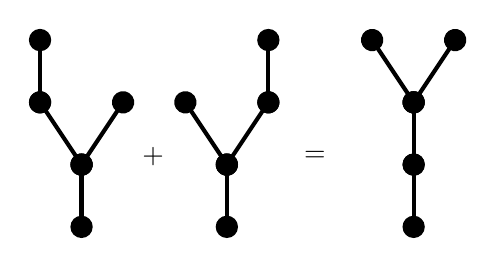
\begin{tikzpicture}[x=0.75pt,y=0.75pt,yscale=-1,xscale=1]
%uncomment if require: \path (0,513); %set diagram left start at 0, and has height of 513

%Straight Lines [id:da5455092391586145] 
\draw [line width=1.5]    (50,90) -- (30,60) ;
\draw [shift={(30,60)}, rotate = 236.31] [color={rgb, 255:red, 0; green, 0; blue, 0 }  ][fill={rgb, 255:red, 0; green, 0; blue, 0 }  ][line width=1.5]      (0, 0) circle [x radius= 4.36, y radius= 4.36]   ;
\draw [shift={(50,90)}, rotate = 236.31] [color={rgb, 255:red, 0; green, 0; blue, 0 }  ][fill={rgb, 255:red, 0; green, 0; blue, 0 }  ][line width=1.5]      (0, 0) circle [x radius= 4.36, y radius= 4.36]   ;
%Straight Lines [id:da552453933363283] 
\draw [line width=1.5]    (50,120) -- (50,90) ;
\draw [shift={(50,90)}, rotate = 270] [color={rgb, 255:red, 0; green, 0; blue, 0 }  ][fill={rgb, 255:red, 0; green, 0; blue, 0 }  ][line width=1.5]      (0, 0) circle [x radius= 4.36, y radius= 4.36]   ;
\draw [shift={(50,120)}, rotate = 270] [color={rgb, 255:red, 0; green, 0; blue, 0 }  ][fill={rgb, 255:red, 0; green, 0; blue, 0 }  ][line width=1.5]      (0, 0) circle [x radius= 4.36, y radius= 4.36]   ;
%Straight Lines [id:da4531423159403052] 
\draw [line width=1.5]    (50,90) -- (70,60) ;
\draw [shift={(70,60)}, rotate = 303.69] [color={rgb, 255:red, 0; green, 0; blue, 0 }  ][fill={rgb, 255:red, 0; green, 0; blue, 0 }  ][line width=1.5]      (0, 0) circle [x radius= 4.36, y radius= 4.36]   ;
\draw [shift={(50,90)}, rotate = 303.69] [color={rgb, 255:red, 0; green, 0; blue, 0 }  ][fill={rgb, 255:red, 0; green, 0; blue, 0 }  ][line width=1.5]      (0, 0) circle [x radius= 4.36, y radius= 4.36]   ;
%Straight Lines [id:da8658811299365152] 
\draw [line width=1.5]    (30,60) -- (30,30) ;
\draw [shift={(30,30)}, rotate = 270] [color={rgb, 255:red, 0; green, 0; blue, 0 }  ][fill={rgb, 255:red, 0; green, 0; blue, 0 }  ][line width=1.5]      (0, 0) circle [x radius= 4.36, y radius= 4.36]   ;
\draw [shift={(30,60)}, rotate = 270] [color={rgb, 255:red, 0; green, 0; blue, 0 }  ][fill={rgb, 255:red, 0; green, 0; blue, 0 }  ][line width=1.5]      (0, 0) circle [x radius= 4.36, y radius= 4.36]   ;
%Straight Lines [id:da9654905799619733] 
\draw [line width=1.5]    (120,90) -- (100,60) ;
\draw [shift={(100,60)}, rotate = 236.31] [color={rgb, 255:red, 0; green, 0; blue, 0 }  ][fill={rgb, 255:red, 0; green, 0; blue, 0 }  ][line width=1.5]      (0, 0) circle [x radius= 4.36, y radius= 4.36]   ;
\draw [shift={(120,90)}, rotate = 236.31] [color={rgb, 255:red, 0; green, 0; blue, 0 }  ][fill={rgb, 255:red, 0; green, 0; blue, 0 }  ][line width=1.5]      (0, 0) circle [x radius= 4.36, y radius= 4.36]   ;
%Straight Lines [id:da12989711620017252] 
\draw [line width=1.5]    (120,120) -- (120,90) ;
\draw [shift={(120,90)}, rotate = 270] [color={rgb, 255:red, 0; green, 0; blue, 0 }  ][fill={rgb, 255:red, 0; green, 0; blue, 0 }  ][line width=1.5]      (0, 0) circle [x radius= 4.36, y radius= 4.36]   ;
\draw [shift={(120,120)}, rotate = 270] [color={rgb, 255:red, 0; green, 0; blue, 0 }  ][fill={rgb, 255:red, 0; green, 0; blue, 0 }  ][line width=1.5]      (0, 0) circle [x radius= 4.36, y radius= 4.36]   ;
%Straight Lines [id:da316004338934887] 
\draw [line width=1.5]    (120,90) -- (140,60) ;
\draw [shift={(140,60)}, rotate = 303.69] [color={rgb, 255:red, 0; green, 0; blue, 0 }  ][fill={rgb, 255:red, 0; green, 0; blue, 0 }  ][line width=1.5]      (0, 0) circle [x radius= 4.36, y radius= 4.36]   ;
\draw [shift={(120,90)}, rotate = 303.69] [color={rgb, 255:red, 0; green, 0; blue, 0 }  ][fill={rgb, 255:red, 0; green, 0; blue, 0 }  ][line width=1.5]      (0, 0) circle [x radius= 4.36, y radius= 4.36]   ;
%Straight Lines [id:da4310585409341743] 
\draw [line width=1.5]    (140,60) -- (140,30) ;
\draw [shift={(140,30)}, rotate = 270] [color={rgb, 255:red, 0; green, 0; blue, 0 }  ][fill={rgb, 255:red, 0; green, 0; blue, 0 }  ][line width=1.5]      (0, 0) circle [x radius= 4.36, y radius= 4.36]   ;
\draw [shift={(140,60)}, rotate = 270] [color={rgb, 255:red, 0; green, 0; blue, 0 }  ][fill={rgb, 255:red, 0; green, 0; blue, 0 }  ][line width=1.5]      (0, 0) circle [x radius= 4.36, y radius= 4.36]   ;
%Straight Lines [id:da5694345020537597] 
\draw [line width=1.5]    (210,60) -- (190,30) ;
\draw [shift={(190,30)}, rotate = 236.31] [color={rgb, 255:red, 0; green, 0; blue, 0 }  ][fill={rgb, 255:red, 0; green, 0; blue, 0 }  ][line width=1.5]      (0, 0) circle [x radius= 4.36, y radius= 4.36]   ;
\draw [shift={(210,60)}, rotate = 236.31] [color={rgb, 255:red, 0; green, 0; blue, 0 }  ][fill={rgb, 255:red, 0; green, 0; blue, 0 }  ][line width=1.5]      (0, 0) circle [x radius= 4.36, y radius= 4.36]   ;
%Straight Lines [id:da353184704299615] 
\draw [line width=1.5]    (210,90) -- (210,60) ;
\draw [shift={(210,60)}, rotate = 270] [color={rgb, 255:red, 0; green, 0; blue, 0 }  ][fill={rgb, 255:red, 0; green, 0; blue, 0 }  ][line width=1.5]      (0, 0) circle [x radius= 4.36, y radius= 4.36]   ;
\draw [shift={(210,90)}, rotate = 270] [color={rgb, 255:red, 0; green, 0; blue, 0 }  ][fill={rgb, 255:red, 0; green, 0; blue, 0 }  ][line width=1.5]      (0, 0) circle [x radius= 4.36, y radius= 4.36]   ;
%Straight Lines [id:da8605408779697565] 
\draw [line width=1.5]    (210,60) -- (230,30) ;
\draw [shift={(230,30)}, rotate = 303.69] [color={rgb, 255:red, 0; green, 0; blue, 0 }  ][fill={rgb, 255:red, 0; green, 0; blue, 0 }  ][line width=1.5]      (0, 0) circle [x radius= 4.36, y radius= 4.36]   ;
\draw [shift={(210,60)}, rotate = 303.69] [color={rgb, 255:red, 0; green, 0; blue, 0 }  ][fill={rgb, 255:red, 0; green, 0; blue, 0 }  ][line width=1.5]      (0, 0) circle [x radius= 4.36, y radius= 4.36]   ;
%Straight Lines [id:da44074219568004036] 
\draw [line width=1.5]    (210,120) -- (210,90) ;
\draw [shift={(210,90)}, rotate = 270] [color={rgb, 255:red, 0; green, 0; blue, 0 }  ][fill={rgb, 255:red, 0; green, 0; blue, 0 }  ][line width=1.5]      (0, 0) circle [x radius= 4.36, y radius= 4.36]   ;
\draw [shift={(210,120)}, rotate = 270] [color={rgb, 255:red, 0; green, 0; blue, 0 }  ][fill={rgb, 255:red, 0; green, 0; blue, 0 }  ][line width=1.5]      (0, 0) circle [x radius= 4.36, y radius= 4.36]   ;

% Text Node
\draw (78,80.4) node [anchor=north west][inner sep=0.75pt]    {$+$};
% Text Node
\draw (156,82.4) node [anchor=north west][inner sep=0.75pt]    {$=$};


\end{tikzpicture}    
\end{center}

which we can recognize as the Leibniz rule. We don't have the $(-1)^{|x|}$ sign here, as it first arises when using the Koszul grading rule when applying these operations to actual elements. The third and final relation is given by 

% The third Stasheff identity for DG algebras using trees



\begin{center}
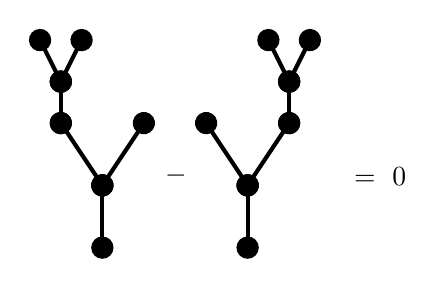
\begin{tikzpicture}[x=0.75pt,y=0.75pt,yscale=-1,xscale=1]
%uncomment if require: \path (0,513); %set diagram left start at 0, and has height of 513

%Straight Lines [id:da5455092391586145] 
\draw [line width=1.5]    (50,90) -- (30,60) ;
\draw [shift={(30,60)}, rotate = 236.31] [color={rgb, 255:red, 0; green, 0; blue, 0 }  ][fill={rgb, 255:red, 0; green, 0; blue, 0 }  ][line width=1.5]      (0, 0) circle [x radius= 4.36, y radius= 4.36]   ;
\draw [shift={(50,90)}, rotate = 236.31] [color={rgb, 255:red, 0; green, 0; blue, 0 }  ][fill={rgb, 255:red, 0; green, 0; blue, 0 }  ][line width=1.5]      (0, 0) circle [x radius= 4.36, y radius= 4.36]   ;
%Straight Lines [id:da552453933363283] 
\draw [line width=1.5]    (50,120) -- (50,90) ;
\draw [shift={(50,90)}, rotate = 270] [color={rgb, 255:red, 0; green, 0; blue, 0 }  ][fill={rgb, 255:red, 0; green, 0; blue, 0 }  ][line width=1.5]      (0, 0) circle [x radius= 4.36, y radius= 4.36]   ;
\draw [shift={(50,120)}, rotate = 270] [color={rgb, 255:red, 0; green, 0; blue, 0 }  ][fill={rgb, 255:red, 0; green, 0; blue, 0 }  ][line width=1.5]      (0, 0) circle [x radius= 4.36, y radius= 4.36]   ;
%Straight Lines [id:da4531423159403052] 
\draw [line width=1.5]    (50,90) -- (70,60) ;
\draw [shift={(70,60)}, rotate = 303.69] [color={rgb, 255:red, 0; green, 0; blue, 0 }  ][fill={rgb, 255:red, 0; green, 0; blue, 0 }  ][line width=1.5]      (0, 0) circle [x radius= 4.36, y radius= 4.36]   ;
\draw [shift={(50,90)}, rotate = 303.69] [color={rgb, 255:red, 0; green, 0; blue, 0 }  ][fill={rgb, 255:red, 0; green, 0; blue, 0 }  ][line width=1.5]      (0, 0) circle [x radius= 4.36, y radius= 4.36]   ;
%Straight Lines [id:da9654905799619733] 
\draw [line width=1.5]    (120,90) -- (100,60) ;
\draw [shift={(100,60)}, rotate = 236.31] [color={rgb, 255:red, 0; green, 0; blue, 0 }  ][fill={rgb, 255:red, 0; green, 0; blue, 0 }  ][line width=1.5]      (0, 0) circle [x radius= 4.36, y radius= 4.36]   ;
\draw [shift={(120,90)}, rotate = 236.31] [color={rgb, 255:red, 0; green, 0; blue, 0 }  ][fill={rgb, 255:red, 0; green, 0; blue, 0 }  ][line width=1.5]      (0, 0) circle [x radius= 4.36, y radius= 4.36]   ;
%Straight Lines [id:da12989711620017252] 
\draw [line width=1.5]    (120,120) -- (120,90) ;
\draw [shift={(120,90)}, rotate = 270] [color={rgb, 255:red, 0; green, 0; blue, 0 }  ][fill={rgb, 255:red, 0; green, 0; blue, 0 }  ][line width=1.5]      (0, 0) circle [x radius= 4.36, y radius= 4.36]   ;
\draw [shift={(120,120)}, rotate = 270] [color={rgb, 255:red, 0; green, 0; blue, 0 }  ][fill={rgb, 255:red, 0; green, 0; blue, 0 }  ][line width=1.5]      (0, 0) circle [x radius= 4.36, y radius= 4.36]   ;
%Straight Lines [id:da316004338934887] 
\draw [line width=1.5]    (120,90) -- (140,60) ;
\draw [shift={(140,60)}, rotate = 303.69] [color={rgb, 255:red, 0; green, 0; blue, 0 }  ][fill={rgb, 255:red, 0; green, 0; blue, 0 }  ][line width=1.5]      (0, 0) circle [x radius= 4.36, y radius= 4.36]   ;
\draw [shift={(120,90)}, rotate = 303.69] [color={rgb, 255:red, 0; green, 0; blue, 0 }  ][fill={rgb, 255:red, 0; green, 0; blue, 0 }  ][line width=1.5]      (0, 0) circle [x radius= 4.36, y radius= 4.36]   ;
%Straight Lines [id:da7774818944643269] 
\draw [line width=1.5]    (30,40) -- (20,20) ;
\draw [shift={(20,20)}, rotate = 243.43] [color={rgb, 255:red, 0; green, 0; blue, 0 }  ][fill={rgb, 255:red, 0; green, 0; blue, 0 }  ][line width=1.5]      (0, 0) circle [x radius= 4.36, y radius= 4.36]   ;
\draw [shift={(30,40)}, rotate = 243.43] [color={rgb, 255:red, 0; green, 0; blue, 0 }  ][fill={rgb, 255:red, 0; green, 0; blue, 0 }  ][line width=1.5]      (0, 0) circle [x radius= 4.36, y radius= 4.36]   ;
%Straight Lines [id:da04997050128847502] 
\draw [line width=1.5]    (30,60) -- (30,40) ;
\draw [shift={(30,40)}, rotate = 270] [color={rgb, 255:red, 0; green, 0; blue, 0 }  ][fill={rgb, 255:red, 0; green, 0; blue, 0 }  ][line width=1.5]      (0, 0) circle [x radius= 4.36, y radius= 4.36]   ;
\draw [shift={(30,60)}, rotate = 270] [color={rgb, 255:red, 0; green, 0; blue, 0 }  ][fill={rgb, 255:red, 0; green, 0; blue, 0 }  ][line width=1.5]      (0, 0) circle [x radius= 4.36, y radius= 4.36]   ;
%Straight Lines [id:da14436077290047278] 
\draw [line width=1.5]    (30,40) -- (40,20) ;
\draw [shift={(40,20)}, rotate = 296.57] [color={rgb, 255:red, 0; green, 0; blue, 0 }  ][fill={rgb, 255:red, 0; green, 0; blue, 0 }  ][line width=1.5]      (0, 0) circle [x radius= 4.36, y radius= 4.36]   ;
\draw [shift={(30,40)}, rotate = 296.57] [color={rgb, 255:red, 0; green, 0; blue, 0 }  ][fill={rgb, 255:red, 0; green, 0; blue, 0 }  ][line width=1.5]      (0, 0) circle [x radius= 4.36, y radius= 4.36]   ;
%Straight Lines [id:da9695689491811674] 
\draw [line width=1.5]    (140,40) -- (130,20) ;
\draw [shift={(130,20)}, rotate = 243.43] [color={rgb, 255:red, 0; green, 0; blue, 0 }  ][fill={rgb, 255:red, 0; green, 0; blue, 0 }  ][line width=1.5]      (0, 0) circle [x radius= 4.36, y radius= 4.36]   ;
\draw [shift={(140,40)}, rotate = 243.43] [color={rgb, 255:red, 0; green, 0; blue, 0 }  ][fill={rgb, 255:red, 0; green, 0; blue, 0 }  ][line width=1.5]      (0, 0) circle [x radius= 4.36, y radius= 4.36]   ;
%Straight Lines [id:da7408167553016403] 
\draw [line width=1.5]    (140,60) -- (140,40) ;
\draw [shift={(140,40)}, rotate = 270] [color={rgb, 255:red, 0; green, 0; blue, 0 }  ][fill={rgb, 255:red, 0; green, 0; blue, 0 }  ][line width=1.5]      (0, 0) circle [x radius= 4.36, y radius= 4.36]   ;
\draw [shift={(140,60)}, rotate = 270] [color={rgb, 255:red, 0; green, 0; blue, 0 }  ][fill={rgb, 255:red, 0; green, 0; blue, 0 }  ][line width=1.5]      (0, 0) circle [x radius= 4.36, y radius= 4.36]   ;
%Straight Lines [id:da11237732756013408] 
\draw [line width=1.5]    (140,40) -- (150,20) ;
\draw [shift={(150,20)}, rotate = 296.57] [color={rgb, 255:red, 0; green, 0; blue, 0 }  ][fill={rgb, 255:red, 0; green, 0; blue, 0 }  ][line width=1.5]      (0, 0) circle [x radius= 4.36, y radius= 4.36]   ;
\draw [shift={(140,40)}, rotate = 296.57] [color={rgb, 255:red, 0; green, 0; blue, 0 }  ][fill={rgb, 255:red, 0; green, 0; blue, 0 }  ][line width=1.5]      (0, 0) circle [x radius= 4.36, y radius= 4.36]   ;

% Text Node
\draw (79,79.4) node [anchor=north west][inner sep=0.75pt]    {$-$};
% Text Node
\draw (170,80.4) node [anchor=north west][inner sep=0.75pt]    {$=\ 0$};


\end{tikzpicture}    
\end{center}

which we recognize as the associativity condition. Here none of the higher arity trees appear, du to the fact that $m_i=0$ for all $i\geq 3$. 